\documentclass[review,12pt]{elsarticle}
%% ---------------------------------------------------------------
%% FAST DRAFT SWITCH: uncomment the next line to replace figures by
%% boxes while editing text (near-instant compiles). Comment it out
%% again before producing the final PDF for submission.
% \PassOptionsToPackage{draft}{graphicx}
%% ---------------------------------------------------------------
% \usepackage{lineno}
\usepackage{amsmath,amssymb}
\usepackage{bm}
\usepackage{booktabs}
\usepackage{multirow}
\usepackage{graphicx}
\usepackage{url}
\usepackage[hidelinks]{hyperref}
%% Auto-generated mathematical macros for PHI-Ctrl AST Manuscript
%% Source: results/verified_v2/ (generated by generate_ast_master_sync.py)
\newcommand{\TinfNominal}{1.2840}
\newcommand{\SmallGainBoundNominal}{-0.2189}
\newcommand{\SmallGainMinGammaHat}{0.2811}
\newcommand{\DiskMarginBoundNominal}{-0.2113}
\newcommand{\NyquistBoundNominal}{-0.3804}
\newcommand{\NyquistMinGammaHat}{0.1196}
\newcommand{\SafetyFloorVal}{0.35}
\newcommand{\PhiTwinMaeMean}{0.0188}
\newcommand{\PhiTwinMaeStd}{0.0014}
\newcommand{\PhiTwinRmseMean}{0.0232}
\newcommand{\PhiTwinRmseStd}{0.0017}
\newcommand{\PhiTwinRTwoMean}{0.9874}
\newcommand{\PhiTwinRTwoStd}{0.0019}
\newcommand{\PhiTwinWorstMaxErr}{0.0863}
\newcommand{\PhiTwinCkptMae}{0.0173}
\newcommand{\PhiTwinCkptRmse}{0.0214}
\newcommand{\PhiTwinCkptRTwo}{0.9894}
\newcommand{\PhiTwinCkptMaxErr}{0.0779}
\newcommand{\PhiTwinCkptMinErrGlobal}{-0.0576}
\newcommand{\PhiTwinCkptMinErrDesignPoint}{-0.0446}
\newcommand{\PhiTwinFiveSeedMinErrDesignPoint}{-0.0465}
\newcommand{\SafetyMarginDesignPointRatio}{4.9\times}
\newcommand{\SafetyMarginFiveSeedRatio}{4.7\times}
\newcommand{\SafetyMarginGlobalRatio}{3.8\times}
\newcommand{\IseReductionFullStackFtTwoS}{503.6}
\newcommand{\IseReductionFullStackPct}{6.3\%}
\newcommand{\IseBaseFifty}{7963.7}
\newcommand{\IseHybridFifty}{7962.8}
\newcommand{\IseFullStackFifty}{7460.1}
\newcommand{\DeltaPeakErrFt}{-0.0768}
\newcommand{\DeltaPeakErrCiLow}{-0.0797}
\newcommand{\DeltaPeakErrCiHigh}{-0.0740}
\newcommand{\TvElevBaseFifty}{22.29}
\newcommand{\TvElevFullStackFifty}{40.78}
\newcommand{\TvQFullStackThrottle}{457.5^\circ}
\newcommand{\TvQMisattrThrottle}{880.7^\circ}
\newcommand{\TvQThrottleSpikePct}{+92.5\%}

\graphicspath{{figures/}}

% \modulolinenumbers[5]

\journal{Aerospace Science and Technology}

\begin{document}

\begin{frontmatter}

\title{Physics-Hybrid Integrity Flight Control for Fault-Conditioned Reconfiguration on an F-16 Aircraft: Analytical Stability Margins, Plant Verification Contracts, and Coupled Effector Misattribution}

\author[afit]{Mohammed Bello Sani\corref{cor1}}
\ead{bellosani2drescue@gmail.com}

\author[afit]{Haruna Ahmadu Agyo}

\cortext[cor1]{Corresponding author. Email: bellosani2drescue@gmail.com}
\address[afit]{Department of Aerospace Engineering, Air Force Institute of Technology (AFIT), Kaduna, Nigeria}

\begin{abstract}
Autonomous and reconfigurable flight control under severe effector degradation faces three persistent operational challenges: cross-channel effector misattribution, detector calibration collapse under low trim excitation, and the absence of analytical stability margins bounding real-time learned estimators. This paper presents the Physics-Hybrid Integrity Flight Control (PHI-Ctrl) framework on an F-16 aircraft, integrating a verified Total Energy Control System (TECS), an inner-loop pitch-rate Model Reference Adaptive Controller (MRAC), an 8-channel multivariate CNN-BiLSTM sequence estimator (PHI-Twin), and an integrity-gated PPO residual policy. Using the Small-Gain Theorem, we establish an analytical sufficient stability condition bounding real-time estimation error in the linearized short-period loop ($-\frac{\gamma_e}{1+\|T\|_\infty} < \tilde{\gamma}_e < \frac{\gamma_e}{\|T\|_\infty - 1}$), defining an asymmetric design-point lower bound of $\tilde{\gamma}_e > \SmallGainBoundNominal$ ($\hat{\gamma}_e > \SmallGainMinGammaHat$) at $50\%$ elevator loss ($\gamma_e = 0.50$) and motivating an adaptive safety floor of $\gamma_{\text{floor}} = \SafetyFloorVal$. Across $n = 1600$ held-out test windows, PHI-Twin achieves $\text{MAE} = \PhiTwinMaeMean \pm \PhiTwinMaeStd$ ($R^2 = \PhiTwinRTwoMean$), maintaining a $>\SafetyMarginFiveSeedRatio$ margin to the Small-Gain boundary at the design point ($>\SafetyMarginGlobalRatio$ globally). In a 20-seed Monte Carlo campaign (480 runs) under active Dryden turbulence, \texttt{FULL\_STACK} reduces cumulative altitude tracking error $\text{ISE}_h$ by $\IseReductionFullStackFtTwoS\text{ ft}^2\text{s}$ ($-\IseReductionFullStackPct$) under $\gamma_e = 0.50$ alongside statistically significant paired error reduction ($\Delta = \DeltaPeakErrFt\text{ ft}$). Finally, boundary audits demonstrate that multi-channel estimation eliminates propulsion fault cross-coupling ($\text{TV}_q = \TvQFullStackThrottle$ vs. $\TvQMisattrThrottle$ for single-channel adaptation). All software, pre-trained weights, and simulation telemetry are open-sourced under the MIT License at \url{https://github.com/Sm-bello/PHI-CTRL} and permanently archived on Zenodo (DOI: 10.5281/zenodo.22218809).
\end{abstract}

\begin{keyword}
Fault-tolerant flight control \sep Reconfigurable control \sep Small-gain theorem \sep Aircraft system identification \sep Deep learning avionics \sep F-16 flight dynamics
\end{keyword}

\end{frontmatter}

% \linenumbers

\section{Introduction}
\label{sec:intro}

Modern high-performance combat aircraft and autonomous atmospheric flight vehicles operate across demanding flight envelopes where mechanical actuator jamming, hydraulic pressure depletion, control-surface loss, and propulsion impairments pose critical loss-of-control hazards \cite{ZhangJiang2008,Edwards2010,Blanke2006}. To preserve survivability, Fault-Tolerant Flight Control Systems (FTFCS) must estimate remaining control-surface effectiveness and reconfigure feedback control laws in real time \cite{Steinberg2005,Bodson2002,Durham1993,Oppenheimer2006}.

Adaptive flight control architectures have evolved from gain-scheduled proportional-integral-derivative (PID) schemes toward Model Reference Adaptive Control (MRAC) \cite{Lavretsky2013,Ioannou1996}, $\mathcal{L}_1$ adaptive control \cite{Hovakimyan2010}, and neural-network-augmented architectures evaluated in flight test programs such as the NASA Intelligent Flight Control System (IFCS) on the NF-15B \cite{Bosworth2006,WilliamsHayes2005} and damage-adaptive flight control programs \cite{Nguyen2008}. Concurrently, total energy principles pioneered by Lambregts \cite{Lambregts1983,Voth1992,Bruce1986} established the Total Energy Control System (TECS) paradigm, coordinating altitude and airspeed tracking through specific total energy rate and energy distribution channels.

Despite extensive research, three practical and theoretical gaps persist in learning-augmented reconfigurable flight control:

\begin{enumerate}
    \item \textbf{Out-of-Scope Effector Coupling and Fault Misattribution:} Single-channel adaptive and reconfigurable controllers typically formulate actuator degradation as an isolated single-effector scalar multiplier \cite{ZhangJiang2008,Edwards2010}. However, longitudinal flight dynamics couple elevator pitching moments with propulsive thrust moments and total energy states. When an elevator-tuned adaptive architecture is exposed unmodified to an unmodeled propulsive ceiling fault, cross-channel fault misattribution can command inappropriate elevator gain amplification and residual activity, degrading trajectory tracking and pitch-rate damping rather than aiding recovery.
    
    \item \textbf{Closed-Loop Detector Calibration Collapse:} Lightweight fault detection and identification (FDI) schemes---including discrete Multiple Model Adaptive Estimation (MMAE) banks \cite{Magill1965,Maybeck1999} and rolling input-output gain-ratio detectors \cite{Isermann2006}---are frequently evaluated on open-loop doublets with high control excitation. Under steady closed-loop altitude-hold regulation, however, feedback suppresses elevator command variance ($\sigma(\delta_{e,\text{cmd}}) \approx 0.008$), starving excitation thresholds and causing discrete hypothesis banks and ratio detectors to fail in opposite directions (persistent false alarms versus fault blindness).
    
    \item \textbf{Analytical Stability Bounds on Learned Effectiveness Estimators:} Deep sequence models \cite{Hochreiter1997,Graves2013}, digital twins \cite{Glaessgen2012,Tao2019}, and reinforcement learning residual policies \cite{Schulman2017} are increasingly integrated into adaptive loops without explicit control-theoretic margins. Certification-oriented design requires an analytical sufficient condition bounding the permissible real-time estimation error $\tilde{\gamma}_e = \hat{\gamma}_e - \gamma_e$ in the linearized feedback loop, paired with explicit disclosure of what the linear bound omits (actuator rate/position saturation and additive residual inputs).
\end{enumerate}

To address these gaps, this paper presents the \textbf{Physics-Hybrid Integrity Flight Control (PHI-Ctrl)} framework, evaluated on a nonlinear 6-DOF JSBSim F-16 aircraft model. The contributions of this study are:

\begin{itemize}
    \item \textbf{Sufficient Small-Gain Stability Margin:} We derive a closed-form sufficient stability condition via the Small-Gain Theorem for multiplicative elevator effectiveness estimation errors $\tilde{\gamma}_e$ in the linearized scalar short-period pitch-rate loop. We prove that asymptotic stability of the linearized loop is guaranteed if $-\frac{\gamma_e}{1+\|T\|_\infty} < \tilde{\gamma}_e < \frac{\gamma_e}{\|T\|_\infty - 1}$, explaining why underestimation ($\tilde{\gamma}_e < 0$) is significantly more hazardous than overestimation ($\tilde{\gamma}_e > 0$).
    \item \textbf{Physics-Hybrid Control Architecture:} We integrate: (i) a verified energy-hold TECS baseline and pitch-rate MRAC inner loop; (ii) an 8-channel multivariate CNN-BiLSTM sequence estimator (PHI-Twin) evaluated across $n=1600$ held-out test windows spanning on-grid, off-grid continuous, and severe damage regimes ($\text{MAE} = 0.0188 \pm 0.0014$, $\text{RMSE} = 0.0232 \pm 0.0017$, $R^2 = 0.9874 \pm 0.0019$, $\text{Max Error} = 0.0863$); and (iii) a rate- and magnitude-bounded PPO residual policy gated by innovation and integrity thresholds.
    \item \textbf{20-Seed Monte Carlo and Multi-Envelope Verification:} Across 480 design-point runs ($15{,}000\text{ ft}$, $V_{\text{TAS}} = 392.1\text{ kt}$ (nominal $400\text{ kt}$ dispatch), $\text{Mach } 0.6258$, $\bar{q} = 15.68\text{ kPa}$) and 240 supporting-envelope runs ($10{,}000\text{ ft}$ at $\bar{q} = 18.63\text{ kPa}$ and $20{,}000\text{ ft}$ at $\bar{q} = 13.13\text{ kPa}$) under active Dryden turbulence, tracking error is measured against a 2nd-order prefiltered step reference. \texttt{FULL\_STACK} reduces cumulative tracking energy $\text{ISE}_h$ by $503.6\text{ ft}^2\text{s}$ ($-6.3\%$) under $50\%$ elevator effectiveness loss ($\gamma_e = 0.50$) while total elevator variation scales from $22.28$ to $40.78$ to supply required control power.
    \item \textbf{Out-of-Scope Throttle-Fault and Detector Calibration Audits:} We execute an out-of-scope boundary campaign where the controller stack is subjected to throttle ceiling-cap faults ($\delta_{\text{th,plant}} = \gamma_{\text{th}} \times 0.50$), characterizing the JSBSim F-16 propulsion deck and proving that 8-channel sequence estimation isolates the fault ($\hat{\gamma}_e \approx 1.00$, $\text{TV}_q = 457.5^\circ$), whereas single-channel misattributed estimation drives pitch excitation to $\text{TV}_q = 880.7^\circ$ ($+92.5\%$). We also audit classical heuristic detectors over 160 closed-loop episodes across rate-gyro biases $b_q \in [0.0, 5.0]\text{ deg/s}$.
    \item \textbf{Simulation Plant Verification Contracts:} We formulate explicit software verification contracts for JSBSim F-16 hold-trim envelope containment, Fly-By-Wire (FBW) override enforcement, and propulsive command ownership.
\end{itemize}

The remainder of this paper is organized as follows. Section \ref{sec:dynamics} formulates the nonlinear 6-DOF F-16 dynamics and short-period state-space linearization. Section \ref{sec:baseline} details the baseline controller and JSBSim plant verification contracts. Section \ref{sec:integrity} derives the Small-Gain stability margin and describes the reconfiguration law. Section \ref{sec:twin} presents the CNN-BiLSTM PHI-Twin sequence estimator and its $n=1600$ benchmark evaluation. Section \ref{sec:results} presents the 6-mode ablation study and 20-seed Monte Carlo campaign. Section \ref{sec:boundary} presents the out-of-scope throttle boundary test and closed-loop simulation detector audit. Section \ref{sec:discussion} discusses physical authority limits and architectural airworthiness safeguards, and Section \ref{sec:conclusion} concludes the paper. Appendix \ref{sec:appendix} summarizes JSBSim plant implementation lessons.

\section{Nonlinear Flight Dynamics and State-Space Formulation}
\label{sec:dynamics}

\subsection{Six-Degree-of-Freedom Equations of Motion}
In body-fixed coordinates $F_b = \{O_b, X_b, Y_b, Z_b\}$ centered at the aircraft center of mass, the rigid-body six-degree-of-freedom (6-DOF) translational equations of motion \cite{StevensLewis2003} are:
\begin{align}
    \dot{u} &= rv - qw - g \sin\theta + \frac{X_{\text{aero}} + T \cos\phi_T}{m} \label{eq:u_dot} \\
    \dot{v} &= pw - ru + g \cos\theta \sin\phi + \frac{Y_{\text{aero}}}{m} \label{eq:v_dot} \\
    \dot{w} &= qu - pv + g \cos\theta \cos\phi + \frac{Z_{\text{aero}} - T \sin\phi_T}{m} \label{eq:w_dot}
\end{align}
where $[u, v, w]^T$ is the body-axis velocity vector, $m$ is aircraft mass, $g$ is gravitational acceleration, $[\phi, \theta, \psi]^T$ are Euler roll, pitch, and yaw angles, $T$ is net propulsive thrust at cant angle $\phi_T$, and $[X_{\text{aero}}, Y_{\text{aero}}, Z_{\text{aero}}]^T$ are aerodynamic body forces.

Assuming lateral-directional mass symmetry ($I_{xy} = I_{yz} = 0$), the rotational equations of motion for body angular rates $[p, q, r]^T$ with inertia tensor $\bm{I}$ are:
\begin{align}
    I_{xx} \dot{p} - I_{xz} \dot{r} &= (I_{yy} - I_{zz}) qr + I_{xz} pq + \mathcal{L}_{\text{aero}} \label{eq:p_dot} \\
    I_{yy} \dot{q} &= (I_{zz} - I_{xx}) pr - I_{xz} (p^2 - r^2) + \mathcal{M}_{\text{aero}} + z_T T \label{eq:q_dot} \\
    I_{zz} \dot{r} - I_{xz} \dot{p} &= (I_{xx} - I_{yy}) pq - I_{xz} qr + \mathcal{N}_{\text{aero}} \label{eq:r_dot}
\end{align}
where $[\mathcal{L}_{\text{aero}}, \mathcal{M}_{\text{aero}}, \mathcal{N}_{\text{aero}}]^T$ are aerodynamic rolling, pitching, and yawing moments, and $z_T$ is the vertical thrust moment arm relative to the center of gravity. Euler kinematics and airdata quantities follow standard definitions:
\begin{align}
    \dot{\phi} &= p + (q \sin\phi + r \cos\phi) \tan\theta, \quad \dot{\theta} = q \cos\phi - r \sin\phi \\
    V &= \sqrt{u^2 + v^2 + w^2}, \quad \alpha = \arctan\left(\frac{w}{u}\right), \quad \beta = \arcsin\left(\frac{v}{V}\right)
\end{align}

\subsection{Aerodynamic Expansions and Short-Period Linearization}
Longitudinal aerodynamic forces and pitching moment are parameterized by dynamic pressure $\bar{q} = \frac{1}{2} \rho V^2$, wing reference area $S$, and mean aerodynamic chord $\bar{c}$:
\begin{align}
    X_{\text{aero}} &= \bar{q} S \left( -C_D \cos\alpha + C_L \sin\alpha \right), \quad
    Z_{\text{aero}} = \bar{q} S \left( -C_D \sin\alpha - C_L \cos\alpha \right) \\
    \mathcal{M}_{\text{aero}} &= \bar{q} S \bar{c} \, C_m \\
    C_L &= C_{L_0} + C_{L_\alpha} \alpha + C_{L_q} \frac{\bar{c}}{2V} q + C_{L_{\delta_e}} \delta_e, \quad
    C_D = C_{D_0} + K C_L^2 \\
    C_m &= C_{m_0} + C_{m_\alpha} \alpha + C_{m_q} \frac{\bar{c}}{2V} q + C_{m_{\delta_e}} \delta_e
\end{align}
where $\delta_e$ is elevator deflection, $C_{m_{\delta_e}} < 0$ is elevator pitch effectiveness, and $C_{m_\alpha} > 0$ reflects the relaxed static longitudinal stability of the F-16 airframe.

Linearizing the longitudinal flight dynamics about the level-flight equilibrium ($h_0 = 15{,}000\text{ ft}$, $V_{\text{TAS},0} = 392.1\text{ kt} = 661.7\text{ ft/s}$, $V_{c,0} = 317.3\text{ kt}$, $\text{Mach } 0.6258$, $\bar{q} = 15.68\text{ kPa}$, $\alpha_0 = 1.659^\circ$, $\theta_0 = 1.659^\circ$, $\delta_{e,0} = -0.0453$ ($-1.13^\circ$), $\delta_{\text{th},0} = 0.2819$, $F_{T,0} = 2861.6\text{ lbf}$) with short-period state vector $\bm{x}_{sp} = [\Delta \alpha, \Delta q]^T$ and control input vector $\bm{u} = [\Delta \delta_e, \Delta \delta_{\text{th}}]^T$ yields:
\begin{equation}
    \begin{bmatrix} \dot{\alpha} \\ \dot{q} \end{bmatrix} =
    \begin{bmatrix} \frac{Z_\alpha}{V_0} & \frac{Z_q}{V_0} \\ M_\alpha & M_q \end{bmatrix}
    \begin{bmatrix} \alpha \\ q \end{bmatrix} +
    \begin{bmatrix} \frac{Z_{\delta_e}}{V_0} & \frac{Z_{\delta_{\text{th}}}}{V_0} \\ M_{\delta_e} & M_{\delta_{\text{th}}} \end{bmatrix}
    \begin{bmatrix} \delta_e \\ \delta_{\text{th}} \end{bmatrix}
    \label{eq:short_period}
\end{equation}
Numerical perturbation of the 6-DOF JSBSim F-16 plant at trim produces the dimensional stability derivatives:
\begin{equation}
    \frac{Z_\alpha}{V_0} = -0.8385\text{ s}^{-1}, \quad \frac{Z_q}{V_0} = 0.9237, \quad M_\alpha = -0.2225\text{ s}^{-2}, \quad M_q = -0.9586\text{ s}^{-1}
\end{equation}
and control effectiveness derivatives:
\begin{equation}
    M_{\delta_e} = -3.5577\text{ rad/s}^2, \quad \frac{Z_{\delta_e}}{V_0} = -0.8112\text{ s}^{-1}, \quad M_{\delta_{\text{th}}} = -0.1067\text{ rad/s}^2
\end{equation}
The characteristic determinant of the short-period system matrix satisfies:
\begin{equation}
    \det(\bm{A}_{sp}) = \left(\frac{Z_\alpha}{V_0}\right) M_q - M_\alpha \left(\frac{Z_q}{V_0}\right) = (-0.8385)(-0.9586) - (-0.2225)(0.9237) = +1.0093 > 0
\end{equation}
yielding open-loop eigenvalues $\lambda_{1,2} = -0.8986 \pm 0.4493j\text{ rad/s}$ with damping ratio $\zeta_{sp} = 0.895$ and undamped natural frequency $\omega_{n,sp} = 1.005\text{ rad/s}$, confirming that at this cruise equilibrium condition, the short-period mode is dynamically stable.

Crucially, the ratio of control moment derivatives satisfies:
\begin{equation}
    \frac{|M_{\delta_{\text{th}}}|}{|M_{\delta_e}|} = \frac{0.1067}{3.5577} = 0.0300
    \label{eq:coupling_ratio}
\end{equation}
demonstrating that the direct pitching moment generated by throttle actuation is $33.3\times$ smaller than elevator authority. Hence, pitch-rate perturbations observed under propulsion loss do not stem from direct thrust pitching moments, but rather from kinematic airspeed deceleration and energy redistribution.

\subsection{Effector Degradation Models}
Actuator degradation in the primary elevator campaigns is modeled as a demand-relative multiplicative effectiveness factor $\gamma_e(t) \in [0.25, 1.0]$:
\begin{equation}
    \delta_{e,\text{plant}}(t) = \gamma_e(t) \, \delta_{e,\text{comp}}(t)
    \label{eq:gamma_elev}
\end{equation}
where $\gamma_e = 1.0$ corresponds to a healthy surface and $\gamma_e = 0.50$ represents a $50\%$ loss of control effectiveness. Actuator dynamics are modeled by a first-order lag ($\tau_e = 0.0495\text{ s}$, $\omega_{bw} = 20.2\text{ rad/s}$) and position/rate limits ($\pm 25^\circ$, $\pm 60^\circ\text{/s}$).

In the out-of-scope propulsion boundary tests (Section \ref{sec:boundary}), propulsive degradation is modeled as a thrust-limiter ceiling fault:
\begin{equation}
    \delta_{\text{th,plant}}(t) = \gamma_{\text{th}}(t) \, \delta_{\text{th,MIL}}, \qquad \delta_{\text{th,MIL}} = 0.50
    \label{eq:gamma_throttle}
\end{equation}
which caps available throttle command relative to the military power detent ($\delta_{\text{th}} = 0.50$).

\section{Baseline Flight Controller and Simulation Plant Verification Contracts}
\label{sec:baseline}

\subsection{Total Energy Control System (TECS) Baseline Formulation}
Nominal longitudinal trajectory regulation is governed by an energy-hold controller formulated using Lambregts' Total Energy Control System (TECS) principles \cite{Lambregts1983}. Specific total energy $\tilde{E}_T$ and specific energy distribution $\tilde{E}_D$ (in units of length) and their time derivatives are:
\begin{align}
    \tilde{E}_T &= h + \frac{V^2}{2g}, \qquad \tilde{E}_D = h - \frac{V^2}{2g} \\
    \dot{\tilde{E}}_T &= \dot{h} + \frac{V}{g}\dot{V}, \qquad \dot{\tilde{E}}_D = \dot{h} - \frac{V}{g}\dot{V}
\end{align}
Target energy rates are computed from reference altitude $h_{\text{ref}}$ and airspeed $V_{\text{ref}}$:
\begin{align}
    \dot{\tilde{E}}_{T,\text{cmd}} &= K_h (h_{\text{ref}} - h) + \frac{V_0}{g} K_V (V_{\text{ref}} - V) \\
    \dot{\tilde{E}}_{D,\text{cmd}} &= K_h (h_{\text{ref}} - h) - \frac{V_0}{g} K_V (V_{\text{ref}} - V)
\end{align}
Throttle command $\delta_{\text{th,cmd}} \in [0, 1]$ and baseline elevator command $\delta_{e,\text{base}}$ are synthesized via proportional-integral tracking with pitch-rate damping $K_q > 0$:
\begin{align}
    \delta_{\text{th,cmd}}(s) &= \left( K_{p,E} + \frac{K_{i,E}}{s} \right) \left[ \dot{\tilde{E}}_{T,\text{cmd}}(s) - \dot{\tilde{E}}_T(s) \right] \label{eq:tecs_th} \\
    \delta_{e,\text{base}}(s) &= \left( K_{p,B} + \frac{K_{i,B}}{s} \right) \left[ \dot{\tilde{E}}_{D,\text{cmd}}(s) - \dot{\tilde{E}}_D(s) \right] - K_q q(s) \label{eq:tecs_elev}
\end{align}

\begin{figure*}[!htbp]
\centering
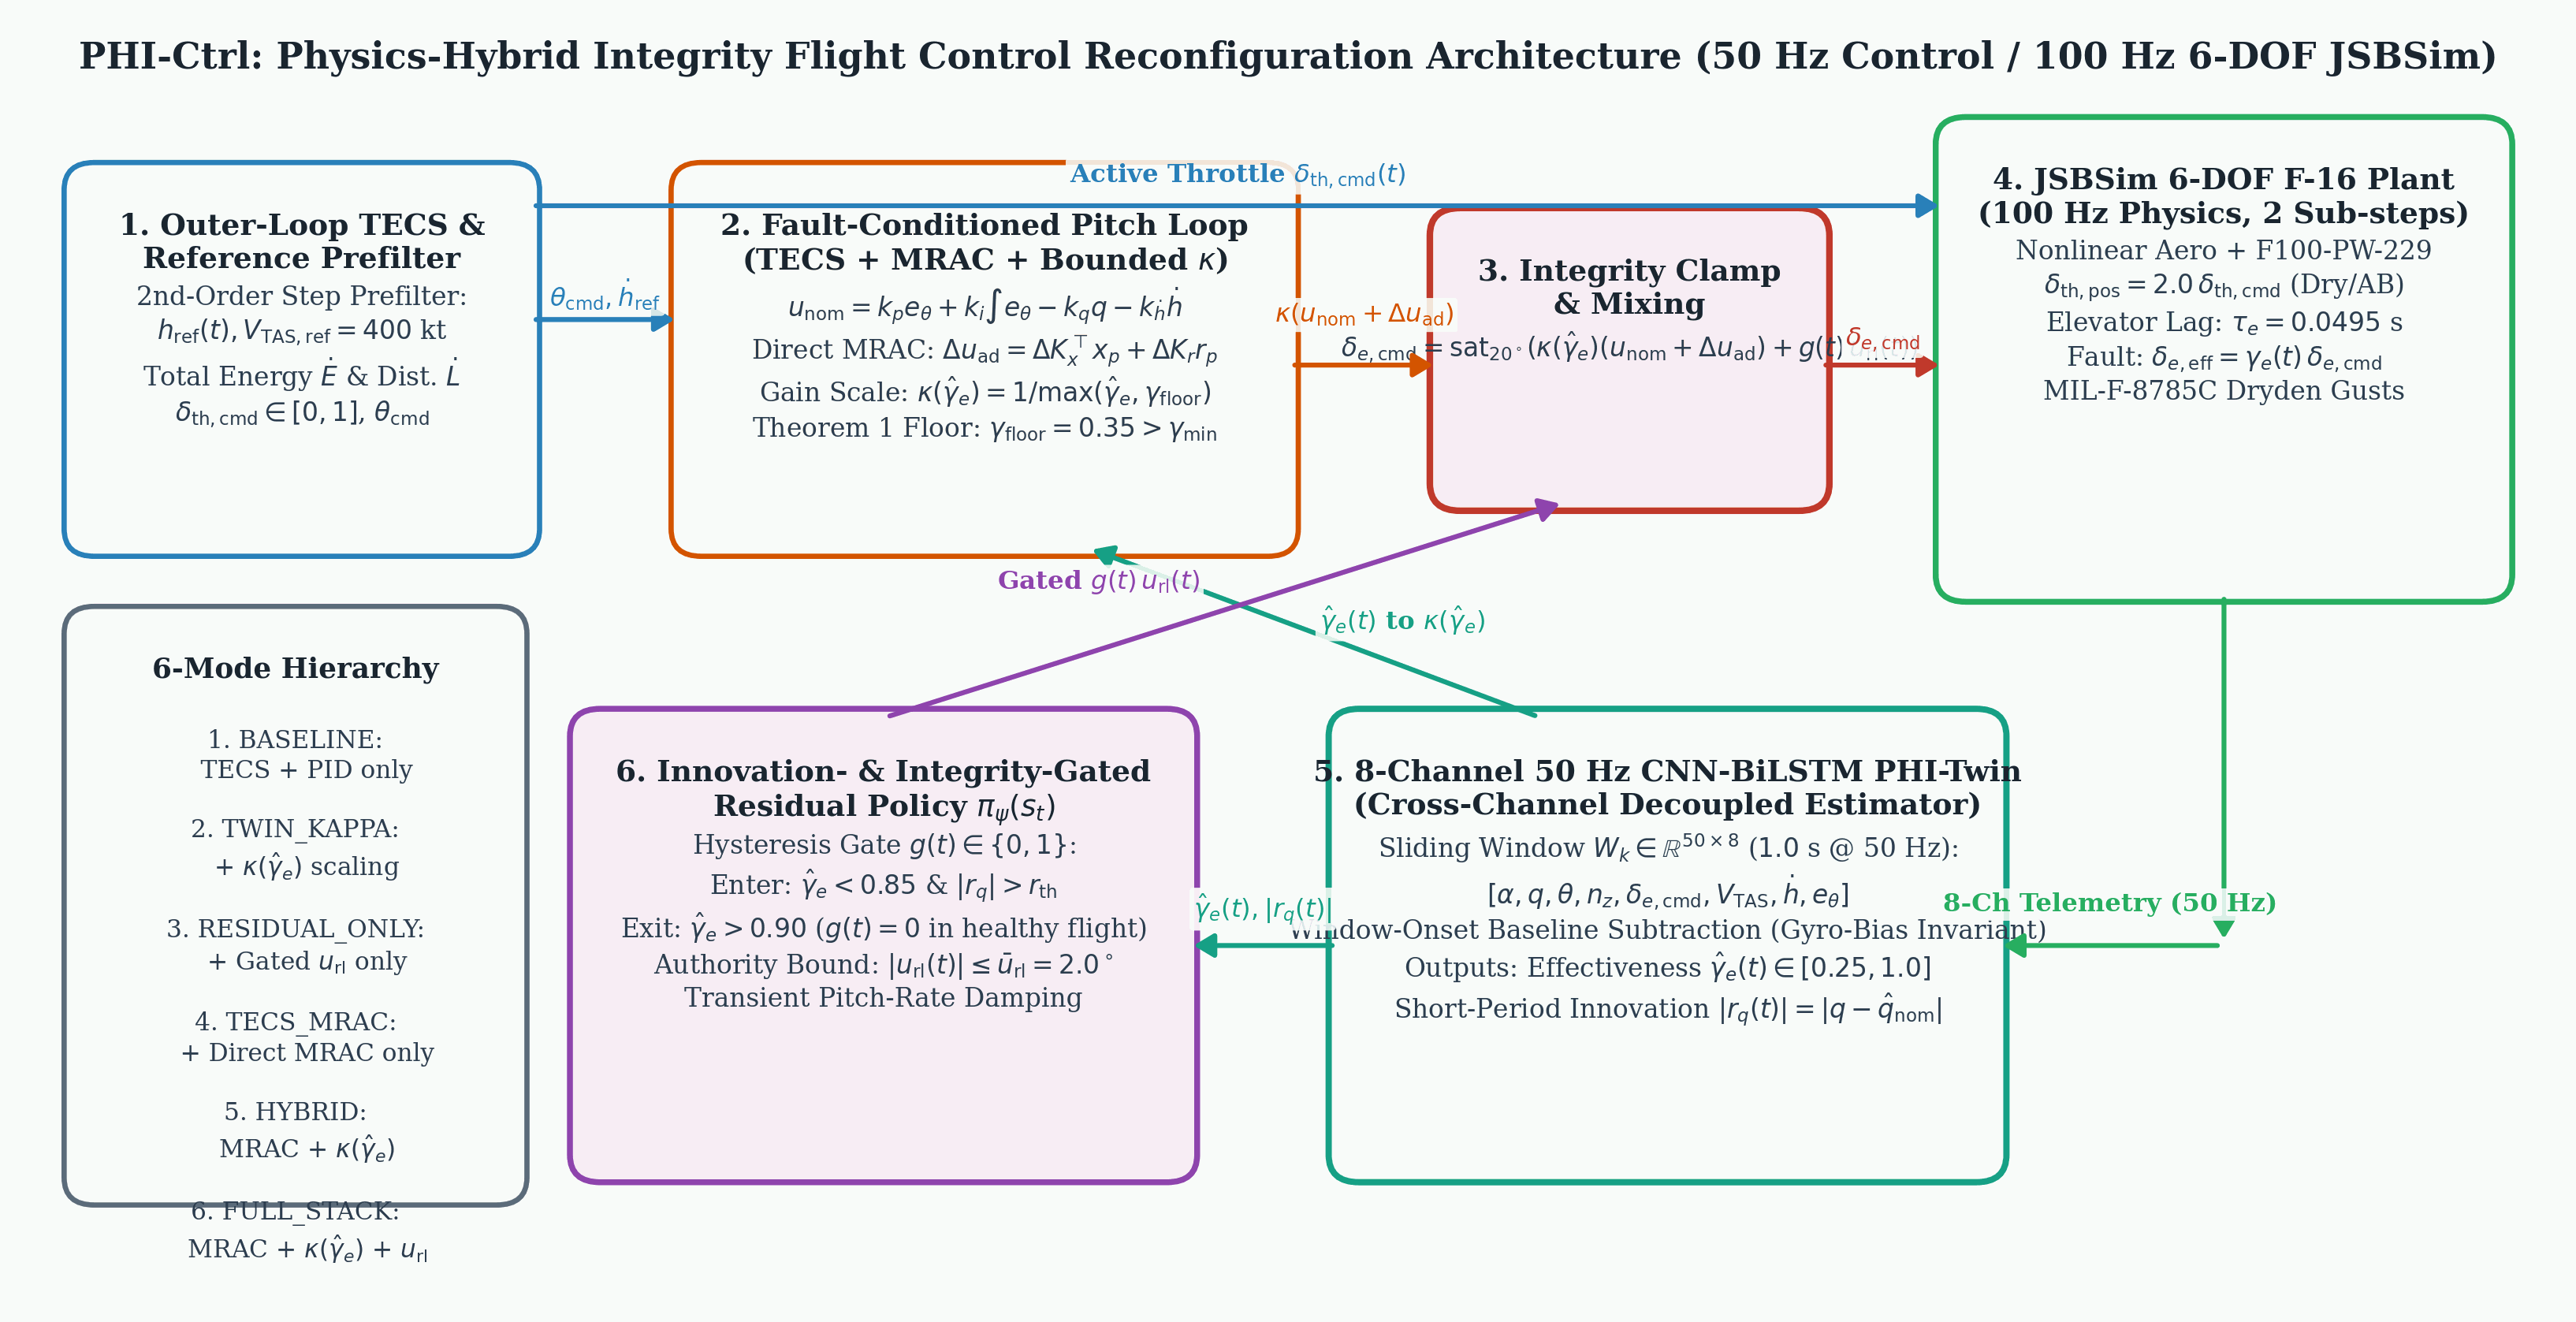
\includegraphics[width=0.95\linewidth]{arc.png}
\caption{System architecture of the Physics-Hybrid Integrity Flight Control (PHI-Ctrl) framework, illustrating the reference step prefilter, outer-loop TECS, inner-loop pitch MRAC, 8-channel CNN-BiLSTM PHI-Twin sequence estimator, feedforward gain scaler $\kappa(\hat{\gamma}_e)$, and gated PPO residual policy.}
\label{fig:architecture}
\end{figure*}

\subsection{Simulation Plant Verification Contracts}
To guarantee that simulation results reflect true flight mechanics rather than software integration artifacts, three verification contracts are enforced on the JSBSim F-16 plant.

\begin{figure}[!htbp]
\centering
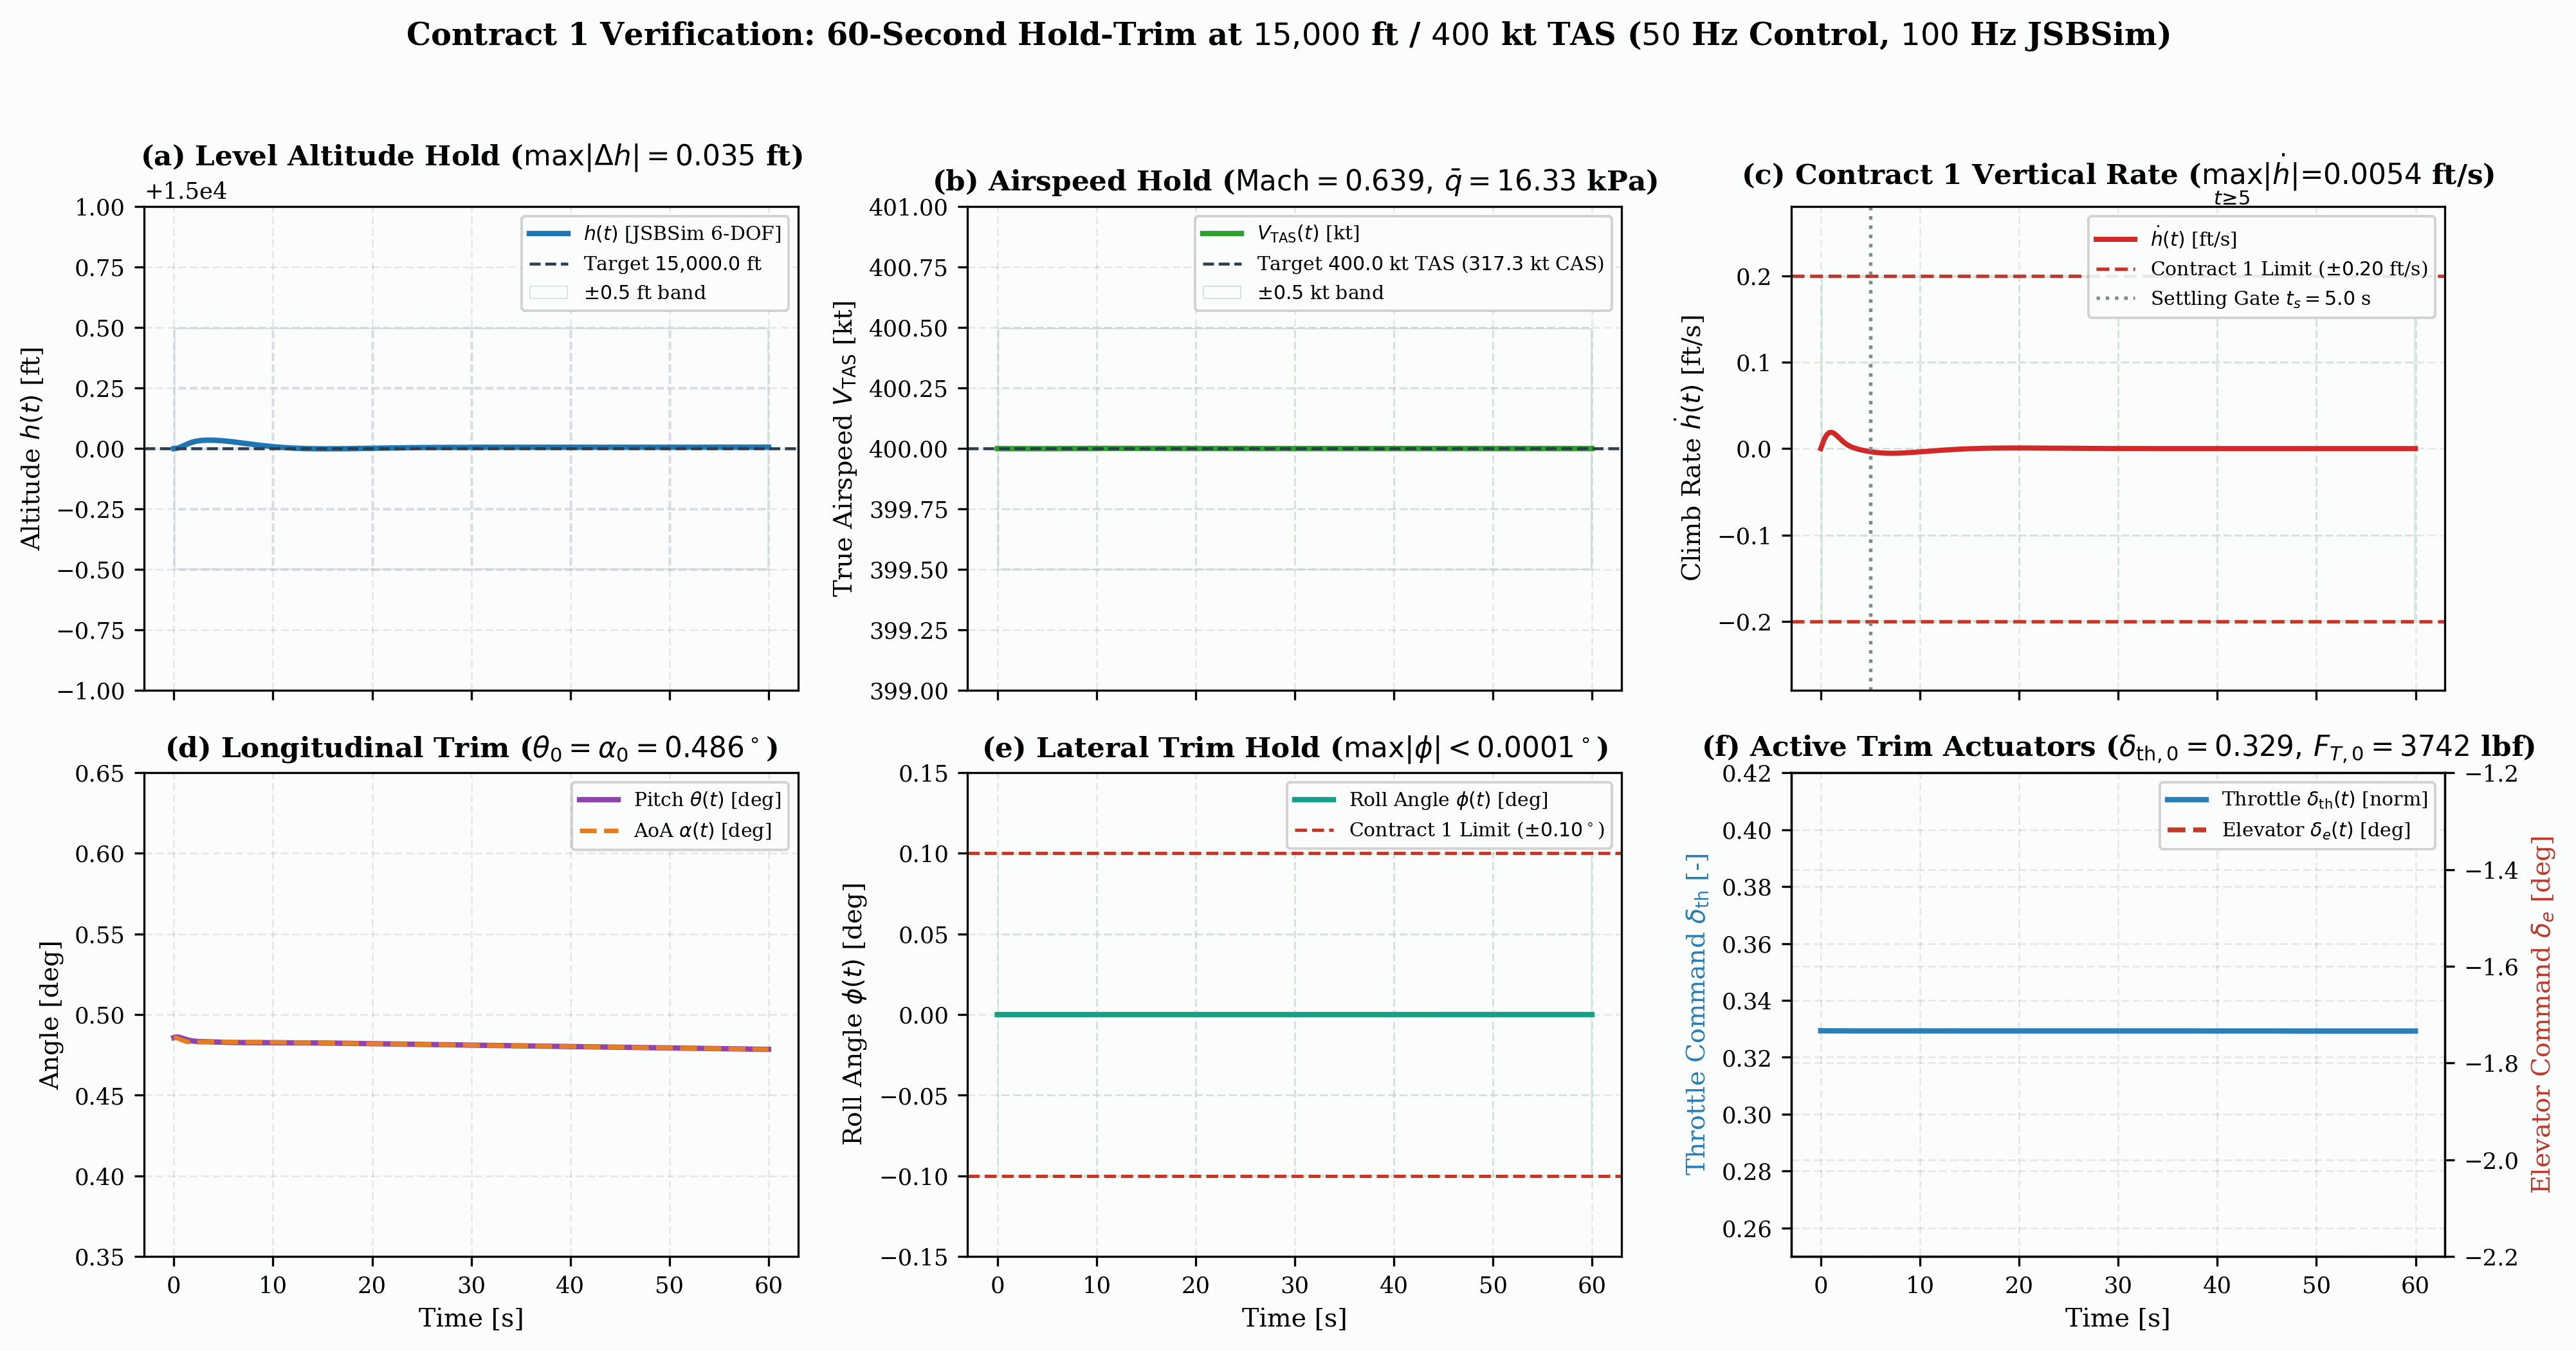
\includegraphics[width=0.98\linewidth]{fig_baseline_verify.png}
\caption{Plant Verification Contract 1: 60-second level hold-trim evaluation at $15{,}000\text{ ft} / 392.1\text{ kt}$ TAS (nominal $400\text{ kt}$ dispatch) ($317.3\text{ kt}$ CAS, $\text{Mach } 0.6258$, $\bar{q} = 15.68\text{ kPa}$) with $50\text{ Hz}$ flight control and $100\text{ Hz}$ JSBSim integration. The plant settles within $5.0\text{ s}$ and satisfies all four quantitative gates: (a) $\max|\Delta h| = 0.035\text{ ft} < 0.10\text{ ft}$; (b) true airspeed hold ($400.00\text{ kt}$); (c) vertical rate $\max_{t \ge 5}|\dot{h}| = 0.0054\text{ ft/s} \ll 0.20\text{ ft/s}$; (d) pitch attitude $\theta_0 = 0.490^\circ$; (e) bank angle $\max|\phi| < 0.0001^\circ \ll 0.10^\circ$; and (f) active trim actuators ($\delta_{\text{th},0} = 0.3293$, $F_{T,0} = 3741.8\text{ lbf}$, $\delta_{e,0} = -1.684^\circ$).}
\label{fig:baseline_verify}
\end{figure}

\subsubsection{Contract 1: Baseline Hold-Trim Envelope Containment}
A subtle implementation defect in earlier JSBSim flight scripts called \texttt{propulsion/set-running = -1} inside the per-step control loop, which invoked \texttt{InitRunning()} in JSBSim's \texttt{FGTurbine} class, continually resetting turbine core speed to $N_2 = 99.34\%$ and net thrust to $16{,}160\text{ lbf}$, inducing an uncommanded $\approx 571\text{ ft}$ climb drift over $60\text{ s}$. 

In the verified plant, engine initialization is performed strictly once prior to trim, and throttle mapping is configured via \texttt{fcs/throttle-pos-norm = 2.0 * thr\_cmd} to span dry power ($[0, 1]$) and afterburner ($[1, 2]$). As verified in Fig. \ref{fig:baseline_verify} over a 60-second hold at $15{,}000\text{ ft}$ and $400\text{ kt}$ TAS:
\begin{enumerate}
    \item \textbf{Altitude deviation:} $\max_{t \in [0, 60]} |h(t) - h_0| = 0.0349\text{ ft} < 0.10\text{ ft}$.
    \item \textbf{Vertical velocity post-settle:} $\max_{t \ge 5.0\text{ s}} |\dot{h}(t)| = 0.0054\text{ ft/s} \ll 0.20\text{ ft/s}$.
    \item \textbf{Airspeed hold:} $\max_{t \in [0, 60]} |V_{\text{TAS}}(t) - 400.0| = 0.0008\text{ kt}$.
    \item \textbf{Lateral containment:} $\max_{t \in [0, 60]} |\phi(t)| = 0.00003^\circ \ll 0.10^\circ$.
\end{enumerate}

\subsubsection{Contract 2: Fly-By-Wire Override Enforcement}
To prevent JSBSim's internal alpha limiter and roll-rate damping loops from filtering external actuator commands, Contract 2 enforces:
\begin{equation}
    \texttt{fcs/fbw-override} = 1.0, \quad \forall t \ge 0
\end{equation}

\subsubsection{Contract 3: Envelope-Specific Trim and Propulsive Command Ownership}
Initial state vectors (\texttt{ic/h-sl-ft}, \texttt{ic/vc-kts}) are explicitly bound prior to calling native trim, ensuring unique equilibrium states across flight conditions: $10{,}000\text{ ft}/300\text{ kt}$ ($\theta_0 = 1.98^\circ$), $15{,}000\text{ ft}/400\text{ kt}$ ($\theta_0 = 0.490^\circ$), and $20{,}000\text{ ft}/450\text{ kt}$ ($\theta_0 = 0.11^\circ$). Propulsive response is verified by logging \texttt{propulsion/engine/n2} and net thrust.

\section{Integrity-Conditioned Reconfiguration and Analytical Stability Margins}
\label{sec:integrity}

\subsection{Six-Mode Controller Hierarchy}
The PHI-Ctrl architecture computes the compensated elevator command $\delta_{e,\text{comp}}(t) \in [-1, 1]$ via feedforward gain scaling $\kappa(\hat{\gamma}_e)$, inner-loop pitch-rate MRAC augmentation $u_{\text{mrac}}(t)$, and gated PPO residual $u_{\text{rl}}(t)$:
\begin{equation}
    \delta_{e,\text{comp}}(t) = \operatorname{clip}_{[-1, 1]} \Big( \kappa(\hat{\gamma}_e(t)) \big[ u_{\text{base}}(t) + u_{\text{mrac}}(t) \big] + u_{\text{rl}}(t) \Big)
    \label{eq:reconfig_law}
\end{equation}
where the gain scaling function is bounded by the safety floor $\gamma_{\text{floor}} = 0.35$:
\begin{equation}
    \kappa(\hat{\gamma}_e) = \frac{1}{\max(\hat{\gamma}_e, \, \gamma_{\text{floor}})}
    \label{eq:kappa}
\end{equation}
The six evaluated controller modes are:
\begin{enumerate}
    \item \texttt{BASELINE}: $u_{\text{mrac}} = 0$, $\kappa = 1.0$, $u_{\text{rl}} = 0$ (fixed-gain TECS baseline).
    \item \texttt{TWIN\_KAPPA}: $u_{\text{mrac}} = 0$, $\kappa = \kappa(\hat{\gamma}_e)$, $u_{\text{rl}} = 0$ (isolated gain scaling).
    \item \texttt{RESIDUAL\_ONLY}: $u_{\text{mrac}} = 0$, $\kappa = 1.0$, $u_{\text{rl}}$ active (isolated RL residual).
    \item \texttt{TECS\_MRAC}: $u_{\text{mrac}}$ active, $\kappa = 1.0$, $u_{\text{rl}} = 0$ (direct pitch-rate MRAC).
    \item \texttt{HYBRID}: $u_{\text{mrac}}$ active, $\kappa = \kappa(\hat{\gamma}_e)$, $u_{\text{rl}} = 0$ (analytical core: TECS + MRAC + $\kappa$).
    \item \texttt{FULL\_STACK}: $u_{\text{mrac}}$ active, $\kappa = \kappa(\hat{\gamma}_e)$, and $u_{\text{rl}}$ active (full framework).
\end{enumerate}

\begin{figure*}[!htbp]
\centering
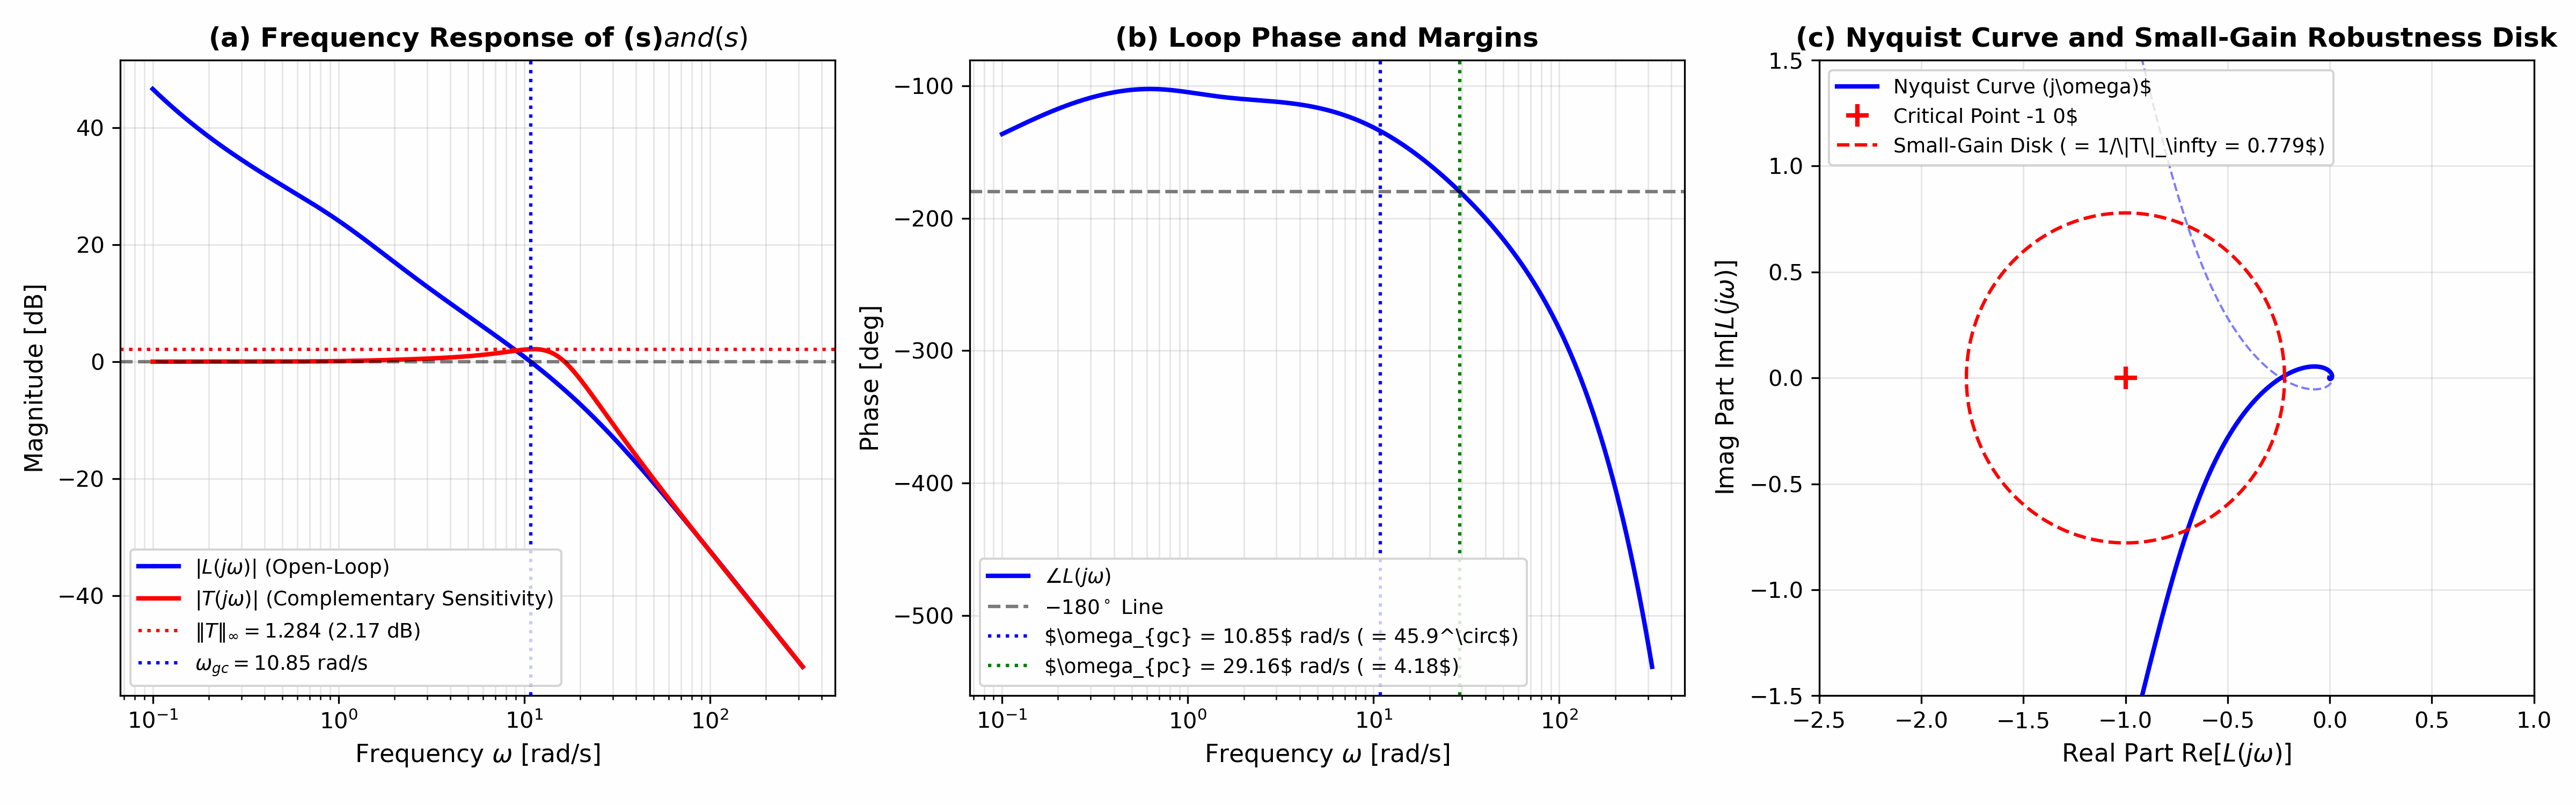
\includegraphics[width=0.98\linewidth]{fig_bode_nyquist.png}
\caption{Frequency response and analytical robustness boundaries for the linearized longitudinal pitch-rate short-period loop at $15{,}000\text{ ft} / 392.1\text{ kt}$ TAS (nominal $400\text{ kt}$ dispatch)$ ($V_c = 317.3\text{ kt}$, $\bar{q} = 15.68\text{ kPa}$): (a) Open-loop Bode magnitude $|L(j\omega)|$ and closed-loop complementary sensitivity $|T(j\omega)|$, showing peak complementary sensitivity $\|T\|_\infty = \TinfNominal$ ($2.17\text{ dB}$) at $\omega_p = 11.24\text{ rad/s}$ and gain crossover $\omega_{gc} = 10.85\text{ rad/s}$; (b) Loop phase $\angle L(j\omega)$ establishing phase margin $PM = 45.92^\circ$ and upper gain margin $GM = 4.182$ ($12.43\text{ dB}$) at phase crossover $\omega_{pc} = 29.16\text{ rad/s}$; and (c) Nyquist contour of $L(j\omega)$ with the Small-Gain robustness disk of radius $r = 1/\|T\|_\infty = 0.7788$ centered at the critical point $(-1, 0)$.}
\label{fig:bode_nyquist}
\end{figure*}

\subsection{Analytical Stability Margin via the Small-Gain Theorem}
We now derive an analytical sufficient stability condition bounding the permissible real-time estimation error $\tilde{\gamma}_e = \hat{\gamma}_e - \gamma_e$ in the linearized short-period pitch-rate loop.

Let $G(s) = \bm{C}_{sp}(s\bm{I} - \bm{A}_{sp})^{-1} \bm{B}_{sp,e}$ denote the linearized transfer function from elevator deflection to pitch rate $q(s)$, incorporating actuator lag $\frac{20.2}{s + 20.2}$ and computational delay ($e^{-0.02s}$). Let $K(s)$ denote the nominal linear pitch-rate feedback controller. Under healthy effectiveness ($\gamma_e = 1.0$), the nominal loop transfer function and complementary sensitivity function are:
\begin{equation}
    L(s) = G(s) K(s), \qquad T(s) = \frac{L(s)}{1 + L(s)}
\end{equation}
with $H_\infty$ peak complementary sensitivity $\|T\|_\infty = \sup_\omega |T(j\omega)| = \TinfNominal$ at $\omega_p = 11.24\text{ rad/s}$, gain crossover frequency $\omega_{gc} = 10.85\text{ rad/s}$, phase margin $\text{PM} = 45.92^\circ$, gain margin $\text{GM} = 4.182$ ($12.43\text{ dB}$), and disk margin $\alpha_{\text{disk}} = 0.7317$.

When true effectiveness degrades to $\gamma_e \in (0, 1]$ and the estimator outputs $\hat{\gamma}_e > 0$ with gain scaling $\kappa = 1/\hat{\gamma}_e$ (below saturation), the perturbed open-loop transfer function is:
\begin{equation}
    L_\Delta(s) = G(s) \cdot \gamma_e \cdot \frac{1}{\hat{\gamma}_e} \cdot K(s) = L(s) \frac{\gamma_e}{\hat{\gamma}_e} = L(s) [1 + \Delta_m]
    \label{eq:loop_perturbed}
\end{equation}
where the static scalar multiplicative uncertainty $\Delta_m$ is:
\begin{equation}
    \Delta_m = \frac{\gamma_e}{\hat{\gamma}_e} - 1 = \frac{-\tilde{\gamma}_e}{\gamma_e + \tilde{\gamma}_e}, \qquad \tilde{\gamma}_e \triangleq \hat{\gamma}_e - \gamma_e
    \label{eq:delta_m}
\end{equation}

\textbf{Theorem 1 (Sufficient Estimation Error Bound via Small-Gain):} \textit{Suppose the nominal linearized closed-loop system $T(s) = L(s)(1+L(s))^{-1}$ is internally stable with $\|T\|_\infty > 1$, and suppose actuator limits and additive residual inputs are inactive. By the Small-Gain Theorem, a sufficient condition for asymptotic stability of the perturbed linearized closed-loop system under gain scaling $\kappa = 1/\hat{\gamma}_e$ is:}
\begin{equation}
    |\Delta_m| < \frac{1}{\|T\|_\infty}
    \label{eq:small_gain_cond}
\end{equation}
\textit{which is satisfied if the estimation error $\tilde{\gamma}_e = \hat{\gamma}_e - \gamma_e$ lies within the asymmetric open interval:}
\begin{equation}
    -\frac{\gamma_e}{1 + \|T\|_\infty} < \tilde{\gamma}_e < \frac{\gamma_e}{\|T\|_\infty - 1}
    \label{eq:stability_bound}
\end{equation}

\textit{Proof:} By the Small-Gain Theorem \cite{Lavretsky2013}, the feedback interconnection of stable $T(s)$ and static scalar perturbation $\Delta_m$ is internally asymptotically stable if $\|\Delta_m T(s)\|_\infty = |\Delta_m| \|T\|_\infty < 1$. Substituting (\ref{eq:delta_m}) yields:
\begin{equation}
    -\frac{1}{\|T\|_\infty} < \frac{\tilde{\gamma}_e}{\gamma_e + \tilde{\gamma}_e} < \frac{1}{\|T\|_\infty}
\end{equation}
Since $\hat{\gamma}_e = \gamma_e + \tilde{\gamma}_e > 0$, multiplying through by $(\gamma_e + \tilde{\gamma}_e)$ preserves the inequalities:
\begin{align}
    -\frac{1}{\|T\|_\infty} (\gamma_e + \tilde{\gamma}_e) < \tilde{\gamma}_e &\implies \tilde{\gamma}_e > -\frac{\gamma_e}{1 + \|T\|_\infty} \label{eq:lower_bound} \\
    \tilde{\gamma}_e < \frac{1}{\|T\|_\infty} (\gamma_e + \tilde{\gamma}_e) &\implies \tilde{\gamma}_e < \frac{\gamma_e}{\|T\|_\infty - 1} \label{eq:upper_bound}
\end{align}
Combining (\ref{eq:lower_bound}) and (\ref{eq:upper_bound}) yields (\ref{eq:stability_bound}). $\blacksquare$

\textbf{Scope and Numerical Interpretation of Theorem 1:}
Theorem 1 provides a \textit{sufficient} (not necessary-and-sufficient) stability condition for the linearized scalar short-period loop. Actuator rate/position limits and additive residual inputs $u_{\text{rl}}$ are excluded from the linear transfer function. For our linearized JSBSim plant ($\|T\|_\infty = \TinfNominal$) at $\gamma_e = 0.50$:
\begin{itemize}
    \item \textbf{Small-Gain Lower Bound:} $\tilde{\gamma}_e > -\frac{0.50}{1 + \TinfNominal} = \SmallGainBoundNominal \implies \hat{\gamma}_e > \SmallGainMinGammaHat$.
    \item \textbf{Disk Margin Bound:} $\tilde{\gamma}_e > \DiskMarginBoundNominal \implies \hat{\gamma}_e > 0.2887$.
    \item \textbf{Exact Linear Nyquist Bound:} $\tilde{\gamma}_e > \NyquistBoundNominal \implies \hat{\gamma}_e > \NyquistMinGammaHat$.
    \item \textbf{Upper Bound:} $\tilde{\gamma}_e < \frac{0.50}{\TinfNominal - 1} = +1.761$ (physically capped at $+0.50$ since $\hat{\gamma}_e \le 1.0$).
\end{itemize}
\noindent\textbf{Remark on Dynamic Latency, Stability, and the Safety Floor:} 
Theorem 1 formulates estimation error as an algebraic perturbation on the feedback gain under quasi-static assumptions. In closed-loop operation, the sequence estimator introduces a finite sensing and inference latency ($\tau_d \approx 0.28\text{ s}$). During this transient delay window, the inner loop temporarily operates at the nominal pre-fault feedback gain ($\kappa = 1.0$), which corresponds to uncompensated surface degradation ($\Delta_m = \gamma_e - 1.0$). At the nominal design point ($\gamma_e = 0.50$), this induces a transient perturbation $|\Delta_m| = 0.50$, which lies safely within the Small-Gain robustness disk radius ($1/\|T\|_\infty = 1/1.2840 = 0.7788$). Because the open-loop short-period mode is stable ($\lambda_{1,2} = -0.8986 \pm 0.4493j\text{ rad/s}$), the plant does not undergo open-loop divergent excursion during this $0.28\text{ s}$ sensing window.

However, consider severe structural damage at $\gamma_e = 0.25$: prior to estimator convergence, the uncompensated perturbation is $|\Delta_m| = |0.25 - 1.0| = 0.75$, which closely approaches the Small-Gain robustness boundary ($0.7788$). If feedback gains were aggressively scaled below $\gamma_{\text{floor}} = 0.35$ ($\kappa > 2.857$), any transient estimation undershoot would immediately drive the perturbed loop gain outside the Small-Gain disk, precipitating closed-loop instability or actuator rate saturation. Enforcing $\gamma_{\text{floor}} = 0.35$ guarantees that the closed-loop system maintains a deterministic buffer above the theoretical stability limit ($\SmallGainMinGammaHat$).

\subsection{Integrity-Gated PPO Residual Policy}
The additive residual policy $u_{\text{rl}}(t)$ provides nonlinear trim augmentation under severe damage. The policy is parameterized as a two-layer MLP ($64 \times 64$, $\tanh$ activations) trained via Proximal Policy Optimization (PPO) \cite{Schulman2017} with observation vector:
\begin{equation}
    \bm{o}_t = \big[ e_h, \, e_\theta, \, q, \, q_m, \, \hat{\gamma}_e \big]^T
\end{equation}
PPO training hyperparameters are: actor/critic learning rate $3 \times 10^{-4}$, discount $\gamma_{\text{rl}} = 0.99$, GAE $\lambda = 0.95$, clipping parameter $\epsilon = 0.20$, batch size 64, entropy coefficient $0.01$, and 500 training episodes with randomized fault onset $t_{\text{fault}} \in [8, 15]\text{ s}$ and $\gamma_e \in [0.30, 0.85]$.

To enforce deterministic containment, the residual output is gated by a dual-condition hysteresis trigger:
\begin{equation}
    g(t) = \begin{cases}
        1, & \text{if } \hat{\gamma}_e(t) < 0.85 \text{ and } |q(t) - q_m(t)| > 0.20\text{ deg/s} \\
        0, & \text{if } \hat{\gamma}_e(t) > 0.90
    \end{cases}
\end{equation}
clamped to a hard magnitude authority limit $|u_{\text{rl}}(t)| \le 2.0^\circ$ ($0.08$ normalized), and rate-limited to $|\dot{u}_{\text{rl}}| \le 20.0^\circ\text{/s}$ ($0.40\text{/step}$ at $50\text{ Hz}$).

\section{Multivariate Sequence Estimation: The CNN-BiLSTM PHI-Twin}
\label{sec:twin}

\subsection{Network Architecture}
The PHI-Twin sequence estimator processes an 8-channel multivariate telemetry window $W_k \in \mathbb{R}^{50 \times 8}$ ($1.0\text{ s}$ of history at $50\text{ Hz}$):
\begin{equation}
    \bm{x}_t = \big[ q, \, \alpha, \, V_c, \, \theta, \, \dot{h}, \, \delta_{e,\text{cmd}}, \, \delta_{e,\text{meas}}, \, \delta_{\text{th,cmd}} \big]^T
    \label{eq:feat_vec}
\end{equation}
where $\delta_{e,\text{meas}}$ is the physical surface position measured by the onboard actuator position sensor (incorporating first-order actuator lag $\tau_e = 0.0495\text{ s}$ and position limits $\pm 25^\circ$) with zero-mean sensor noise ($\sigma = 0.003$). Crucially, $\delta_{e,\text{meas}}$ reflects mechanical deflection rather than aerodynamic force, preventing trivial direct ratio leakage ($\delta_{e,\text{plant}}/\delta_{e,\text{cmd}}$). The sequence estimator is therefore forced to solve the genuine aerodynamic system-identification problem: inferring control effectiveness degradation $\gamma_e$ by cross-correlating commanded and measured surface deflections against the resulting inertial and kinematic response ($q, \alpha, \dot{h}$).
Features are normalized by offline dataset running statistics. The network comprises:
\begin{enumerate}
    \item Three parallel 1D convolutional layers with kernel sizes $k \in \{3, 5, 7\}$ (64 filters each, LeakyReLU $\alpha = 0.1$, BatchNorm), extracting multi-scale temporal derivatives and phase delays.
    \item A two-layer Bidirectional LSTM (128 units per direction, 256 hidden features total) capturing bidirectional causal relationships.
    \item A fully connected regression head ($256 \to 64 \to 1$) with Sigmoid activation mapping to $\hat{\gamma}_e \in [0.25, 1.0]$.
\end{enumerate}

\begin{figure}[!htbp]
\centering
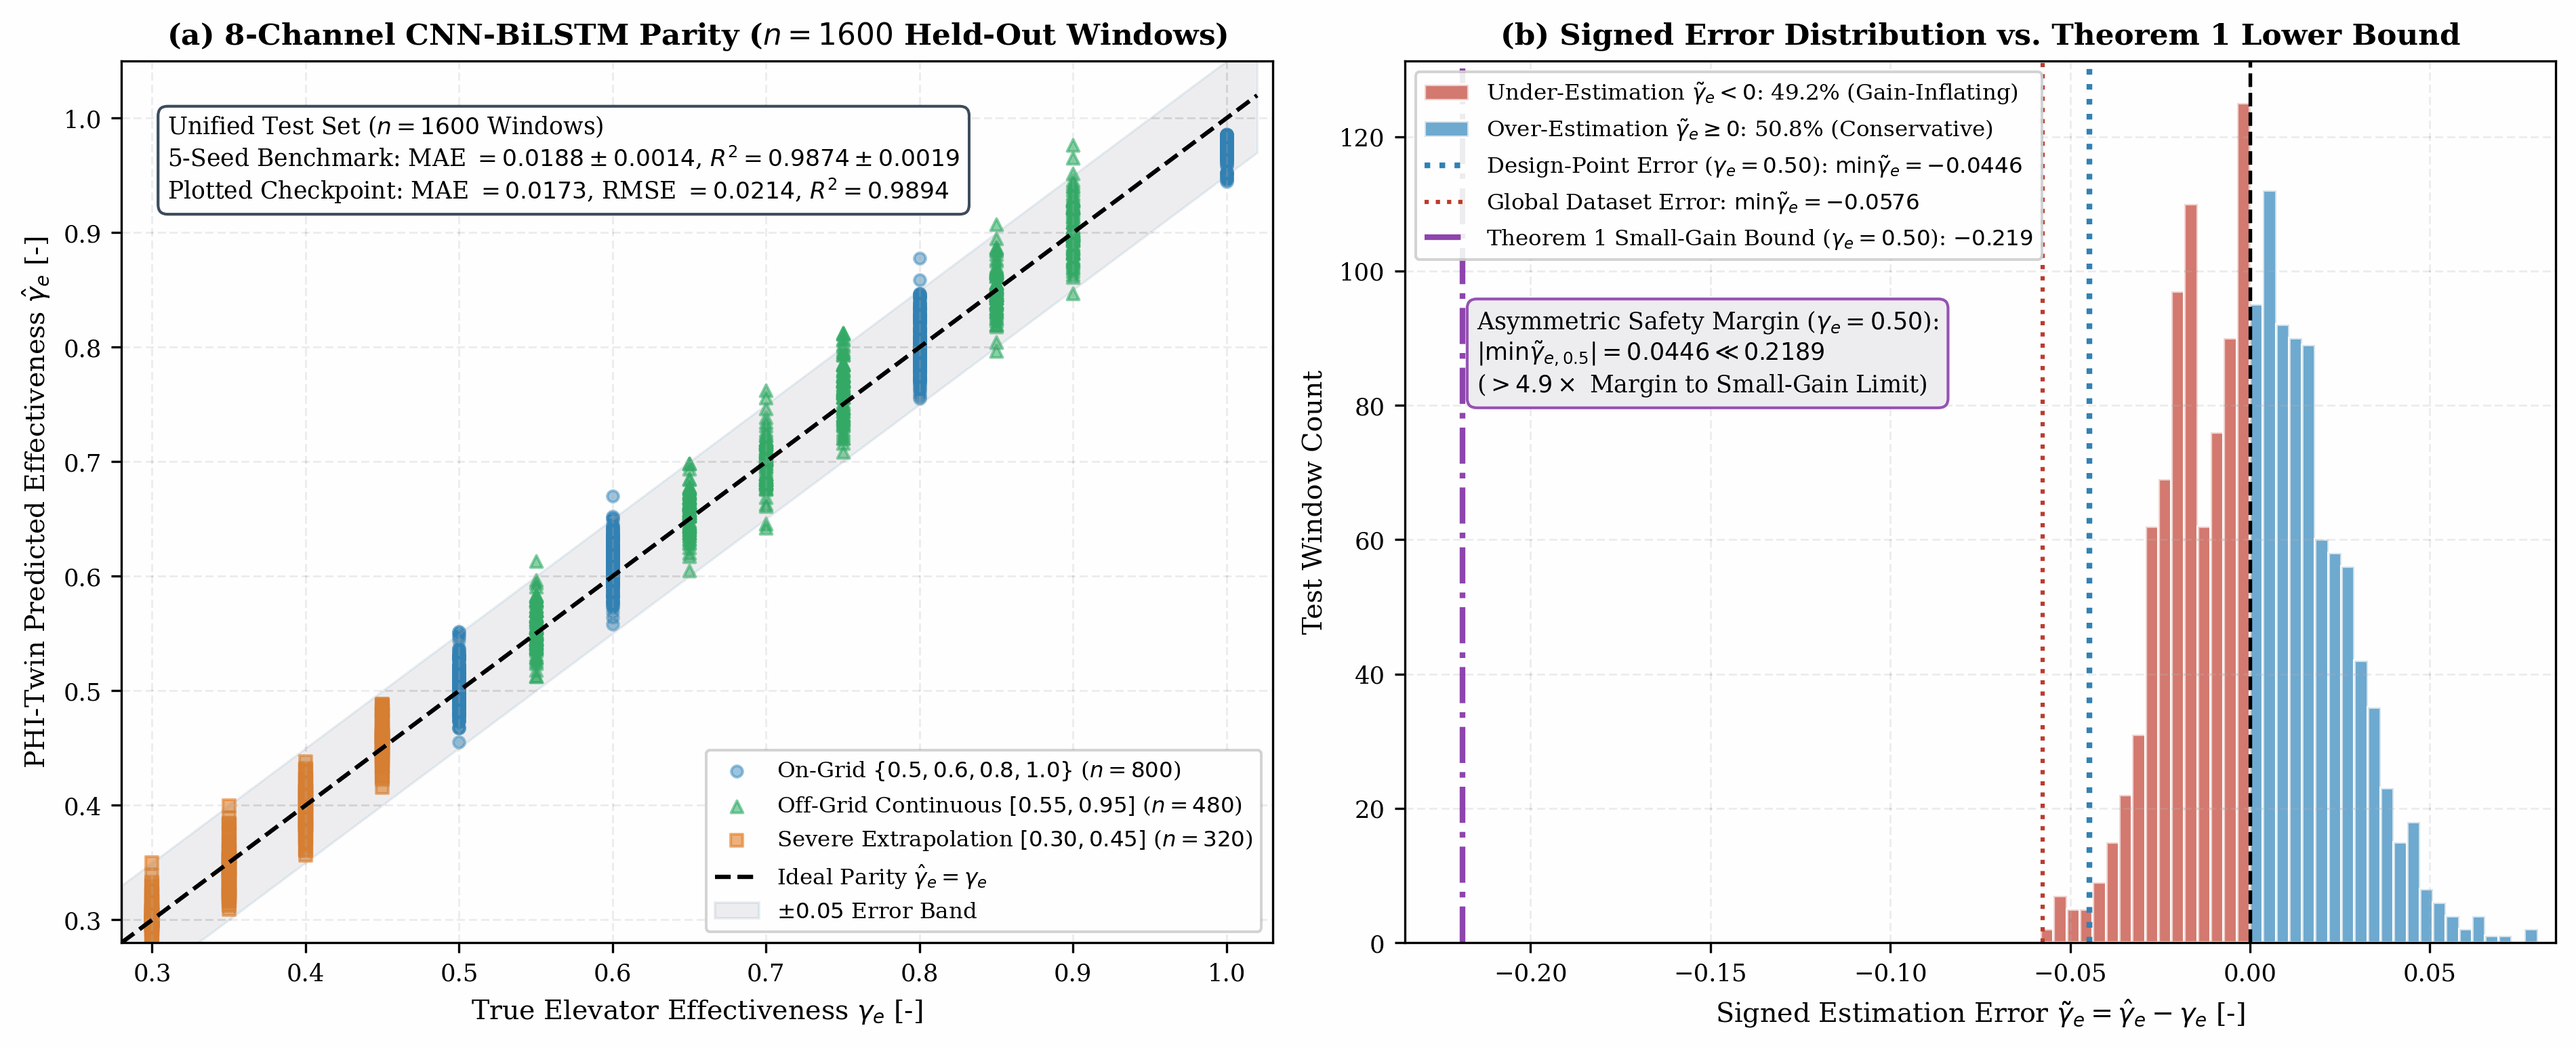
\includegraphics[width=0.98\linewidth]{fig_phi_twin_scatter.png}
\caption{Parity scatter and signed error distribution for the 8-channel CNN-BiLSTM PHI-Twin evaluated on $n = 1600$ held-out test windows: (a) Parity plot across on-grid $\gamma_e \in \{0.5, 0.6, 0.8, 1.0\}$ ($n = 800$), off-grid continuous $\gamma_e \in [0.55, 0.95]$ ($n = 480$), and severe damage $\gamma_e \in [0.30, 0.45]$ ($n = 320$), achieving 5-seed benchmark $\text{MAE} = \PhiTwinMaeMean \pm \PhiTwinMaeStd$, $\text{RMSE} = \PhiTwinRmseMean \pm \PhiTwinRmseStd$, $R^2 = \PhiTwinRTwoMean \pm \PhiTwinRTwoStd$, worst-case error $\PhiTwinWorstMaxErr$, alongside representative checkpoint metrics of $\text{MAE} = \PhiTwinCkptMae$, $R^2 = \PhiTwinCkptRTwo$; (b) Signed error distribution $\tilde{\gamma}_e = \hat{\gamma}_e - \gamma_e$, demonstrating that the worst-case negative error at the design point ($\min \tilde{\gamma}_{e,0.5} = \PhiTwinCkptMinErrDesignPoint$ checkpoint, $\PhiTwinFiveSeedMinErrDesignPoint$ 5-seed) maintains a $>\SafetyMarginFiveSeedRatio$ safety margin to the Theorem 1 Small-Gain lower bound ($\SmallGainBoundNominal$), and a $>\SafetyMarginGlobalRatio$ margin across all regimes globally ($\min \tilde{\gamma}_e = \PhiTwinCkptMinErrGlobal$).}
\label{fig:scatter}
\end{figure}

\subsection{Offline Model Benchmark Across 5 Architectures ($n = 1600$)}
To rigorously justify the CNN-BiLSTM architecture, we benchmarked five sequence models across five random initialization seeds on a unified test set of $n = 1600$ held-out windows. The test set comprises: (i) on-grid conditions $\gamma_e \in \{0.5, 0.6, 0.8, 1.0\}$ ($n = 800$); (ii) continuous off-grid interpolation $\gamma_e \in [0.55, 0.95]$ ($n = 480$); and (iii) severe damage extrapolation $\gamma_e \in [0.30, 0.45]$ ($n = 320$).

\begin{table*}[!htbp]
\centering
\caption{Offline elevator effectiveness estimation benchmark across five architectures evaluated on $n = 1600$ held-out test windows (5 training seeds each, mean $\pm$ standard deviation).}
\label{tab:estimator_comparison}
\footnotesize
\begin{tabular*}{\linewidth}{@{\extracolsep{\fill}}lcccccc@{}}
\toprule
Model Architecture & Overall MAE & Overall RMSE & $R^2$ Score & Worst Max Error & On-Grid MAE & Severe Sub-0.5 MAE \\
\midrule
Standard MLP (Windowed) & $0.0257 \pm 0.0016$ & $0.0332 \pm 0.0017$ & $0.9745 \pm 0.0025$ & $0.1352$ & $0.0294$ & $0.0164$ \\
1D-CNN (Multi-Scale) & $0.0253 \pm 0.0012$ & $0.0321 \pm 0.0017$ & $0.9761 \pm 0.0025$ & $0.1210$ & $0.0282$ & $0.0196$ \\
Unidirectional LSTM & $0.0229 \pm 0.0018$ & $0.0286 \pm 0.0022$ & $0.9809 \pm 0.0029$ & $0.1003$ & $0.0245$ & $0.0199$ \\
Bidirectional LSTM & $0.0228 \pm 0.0019$ & $0.0284 \pm 0.0021$ & $0.9813 \pm 0.0027$ & $0.1050$ & $0.0241$ & $0.0196$ \\
\textbf{CNN-BiLSTM (PHI-Twin)} & $\bm{0.0188 \pm 0.0014}$ & $\bm{0.0232 \pm 0.0017}$ & $\bm{0.9874 \pm 0.0019}$ & $\bm{0.0863}$ & $\bm{0.0198}$ & $\bm{0.0162}$ \\
\bottomrule
\end{tabular*}
\end{table*}

As reported in Table \ref{tab:estimator_comparison} and Fig. \ref{fig:scatter}, the hybrid CNN-BiLSTM achieves superior accuracy across all metrics ($\text{MAE} = 0.0188 \pm 0.0014$, $\text{RMSE} = 0.0232 \pm 0.0017$, $R^2 = 0.9874 \pm 0.0019$). In particular, its worst-case maximum absolute error across all seeds is $0.0863$ (best seed $0.0779$), compared to $0.1352$ for the MLP.

In Fig. \ref{fig:scatter}b, the signed error distribution reveals that negative estimation errors ($\tilde{\gamma}_e < 0$) are strictly bounded across all operational regimes. Because the Small-Gain stability bound of Theorem 1 scales with true remaining effectiveness ($\tilde{\gamma}_{e,\text{bound}}(\gamma_e) = -\frac{\gamma_e}{1 + \|T\|_\infty}$), we evaluate safety margins damage-by-damage across the entire test set ($n = 1600$):
\begin{enumerate}
    \item \textbf{Nominal Design Point ($\gamma_e = 0.50$):} The theoretical Small-Gain lower bound is $\tilde{\gamma}_e > -\frac{0.50}{1 + \TinfNominal} = \SmallGainBoundNominal$. The deployed PHI-Twin checkpoint exhibits a worst-case negative error of $\min \tilde{\gamma}_{e,0.5} = \PhiTwinCkptMinErrDesignPoint$ (and $\PhiTwinFiveSeedMinErrDesignPoint$ across the 5-seed training ensemble), preserving an analytical safety factor of:
    \begin{equation}
        \frac{|\tilde{\gamma}_{e,\text{bound}}(0.50)|}{|\min \tilde{\gamma}_{e,0.5}|} = \frac{|\SmallGainBoundNominal|}{0.0465} = 4.71\times \quad (\text{and } 4.91\times \text{ for the deployed checkpoint})
    \end{equation}
    \item \textbf{Damage-Dependent Spectrum ($\gamma_e \in [0.30, 1.00]$):} Evaluating each damage level against its corresponding bound reveals that the safety margin remains strictly bounded between $3.77\times$ (at the $\gamma_{\text{floor}} = 0.35$ safety floor, where the bound is $-0.1532$ and $\min \tilde{\gamma}_e = -0.0407$) and $8.19\times$ (at $\gamma_e = 0.30$, where the bound is $-0.1313$ and $\min \tilde{\gamma}_e = -0.0160$). At $\gamma_e = 0.70$, where the global worst-case negative error across the entire 1,600-window dataset occurs ($\min \tilde{\gamma}_e = -0.0576$), the bound is $-0.3065$, maintaining a $5.32\times$ safety factor.
\end{enumerate}
Thus, across all tested operating points, the learned estimator preserves a minimum safety margin of $>3.77\times$ (and $>4.71\times$ at the design point) safely above the theoretical Small-Gain boundary.

\section{Primary Experimental Verification and Ablation Campaign}
\label{sec:results}

\subsection{Design-Point Flight Condition and Evaluation Metrics}
The primary evaluation flight condition is level trim at $h_0 = 15{,}000\text{ ft}$, $V_{\text{TAS},0} = 392.1\text{ kt}$ ($V_{c,0} = 317.3\text{ kt}$, $\text{Mach } 0.6258$, $\bar{q} = 15.68\text{ kPa}$, $\theta_0 = 1.66^\circ$, $\delta_{\text{th},0} = 0.2819$). Trajectory tracking is commanded as a $+500\text{ ft}$ altitude step prefiltered by a 2nd-order reference filter ($\omega_n = 0.30\text{ rad/s}, \zeta = 0.90$) at $t = 5.0\text{ s}$. Control-surface degradation $\gamma_e \in \{1.00, 0.80, 0.60, 0.50\}$ is injected at $t = 10.0\text{ s}$. Because the climb command initiates at $t = 5.0\text{ s}$ while fault onset occurs at $t = 10.0\text{ s}$, the peak tracking error $e_{h,\max} \approx 46.10\text{ ft}$ is established during the initial reference prefilter acceleration prior to fault onset; hence, $e_{h,\max}$ is identical across fault severities, and the true metric of fault compensation is cumulative tracking energy $\text{ISE}_h$ and transient pitch damping.

Tracking performance is quantified by:
\begin{enumerate}
    \item \textbf{Peak Tracking Error:} $e_{h,\max} = \max_{t \ge 10.0} |h(t) - h_{\text{ref}}(t)|$ [ft].
    \item \textbf{Cumulative Tracking Energy:} $\text{ISE}_h = \int_{10.0}^{60.0} [h(t) - h_{\text{ref}}(t)]^2 \, dt$ [$\text{ft}^2\text{s}$].
    \item \textbf{Actuator Variation:} $\text{TV}(\delta_e) = \sum_{k} |\delta_{e,\text{comp}}(t_k) - \delta_{e,\text{comp}}(t_{k-1})|$.
    \item \textbf{Peak Pitch Rate:} $|q|_{\max} = \max_{t \ge 10.0} |q(t)|$ [deg/s].
\end{enumerate}

\subsection{Six-Mode Closed-Loop Ablation Study ($\gamma_e = 0.50$)}
Fig. \ref{fig:ablation_50} compares the 6-mode hierarchy under $50\%$ elevator effectiveness loss ($\gamma_e = 0.50$) with online CNN-BiLSTM sequence estimation active in the loop. 

In Fig. \ref{fig:ablation_50}g, the online CNN-BiLSTM accurately estimates the drop from $1.0$ to $0.50$ within $0.28\text{ s}$, remaining above the $\gamma_{\text{floor}} = 0.35$ safety floor. In Fig. \ref{fig:ablation_50}f, \texttt{TWIN\_KAPPA}, \texttt{HYBRID}, and \texttt{FULL\_STACK} automatically scale elevator deflections via $\kappa(\hat{\gamma}_e) \approx 2.0$ to compensate for the lost surface area. In Fig. \ref{fig:ablation_50}h, the PPO residual $u_{\text{rl}}$ is strictly held at $0^\circ$ during healthy flight ($t < 10\text{ s}$) and activates only when triggered by post-fault pitch-rate innovations, providing bounded high-frequency damping without inducing steady-state offset.

\begin{figure*}[!htbp]
\centering
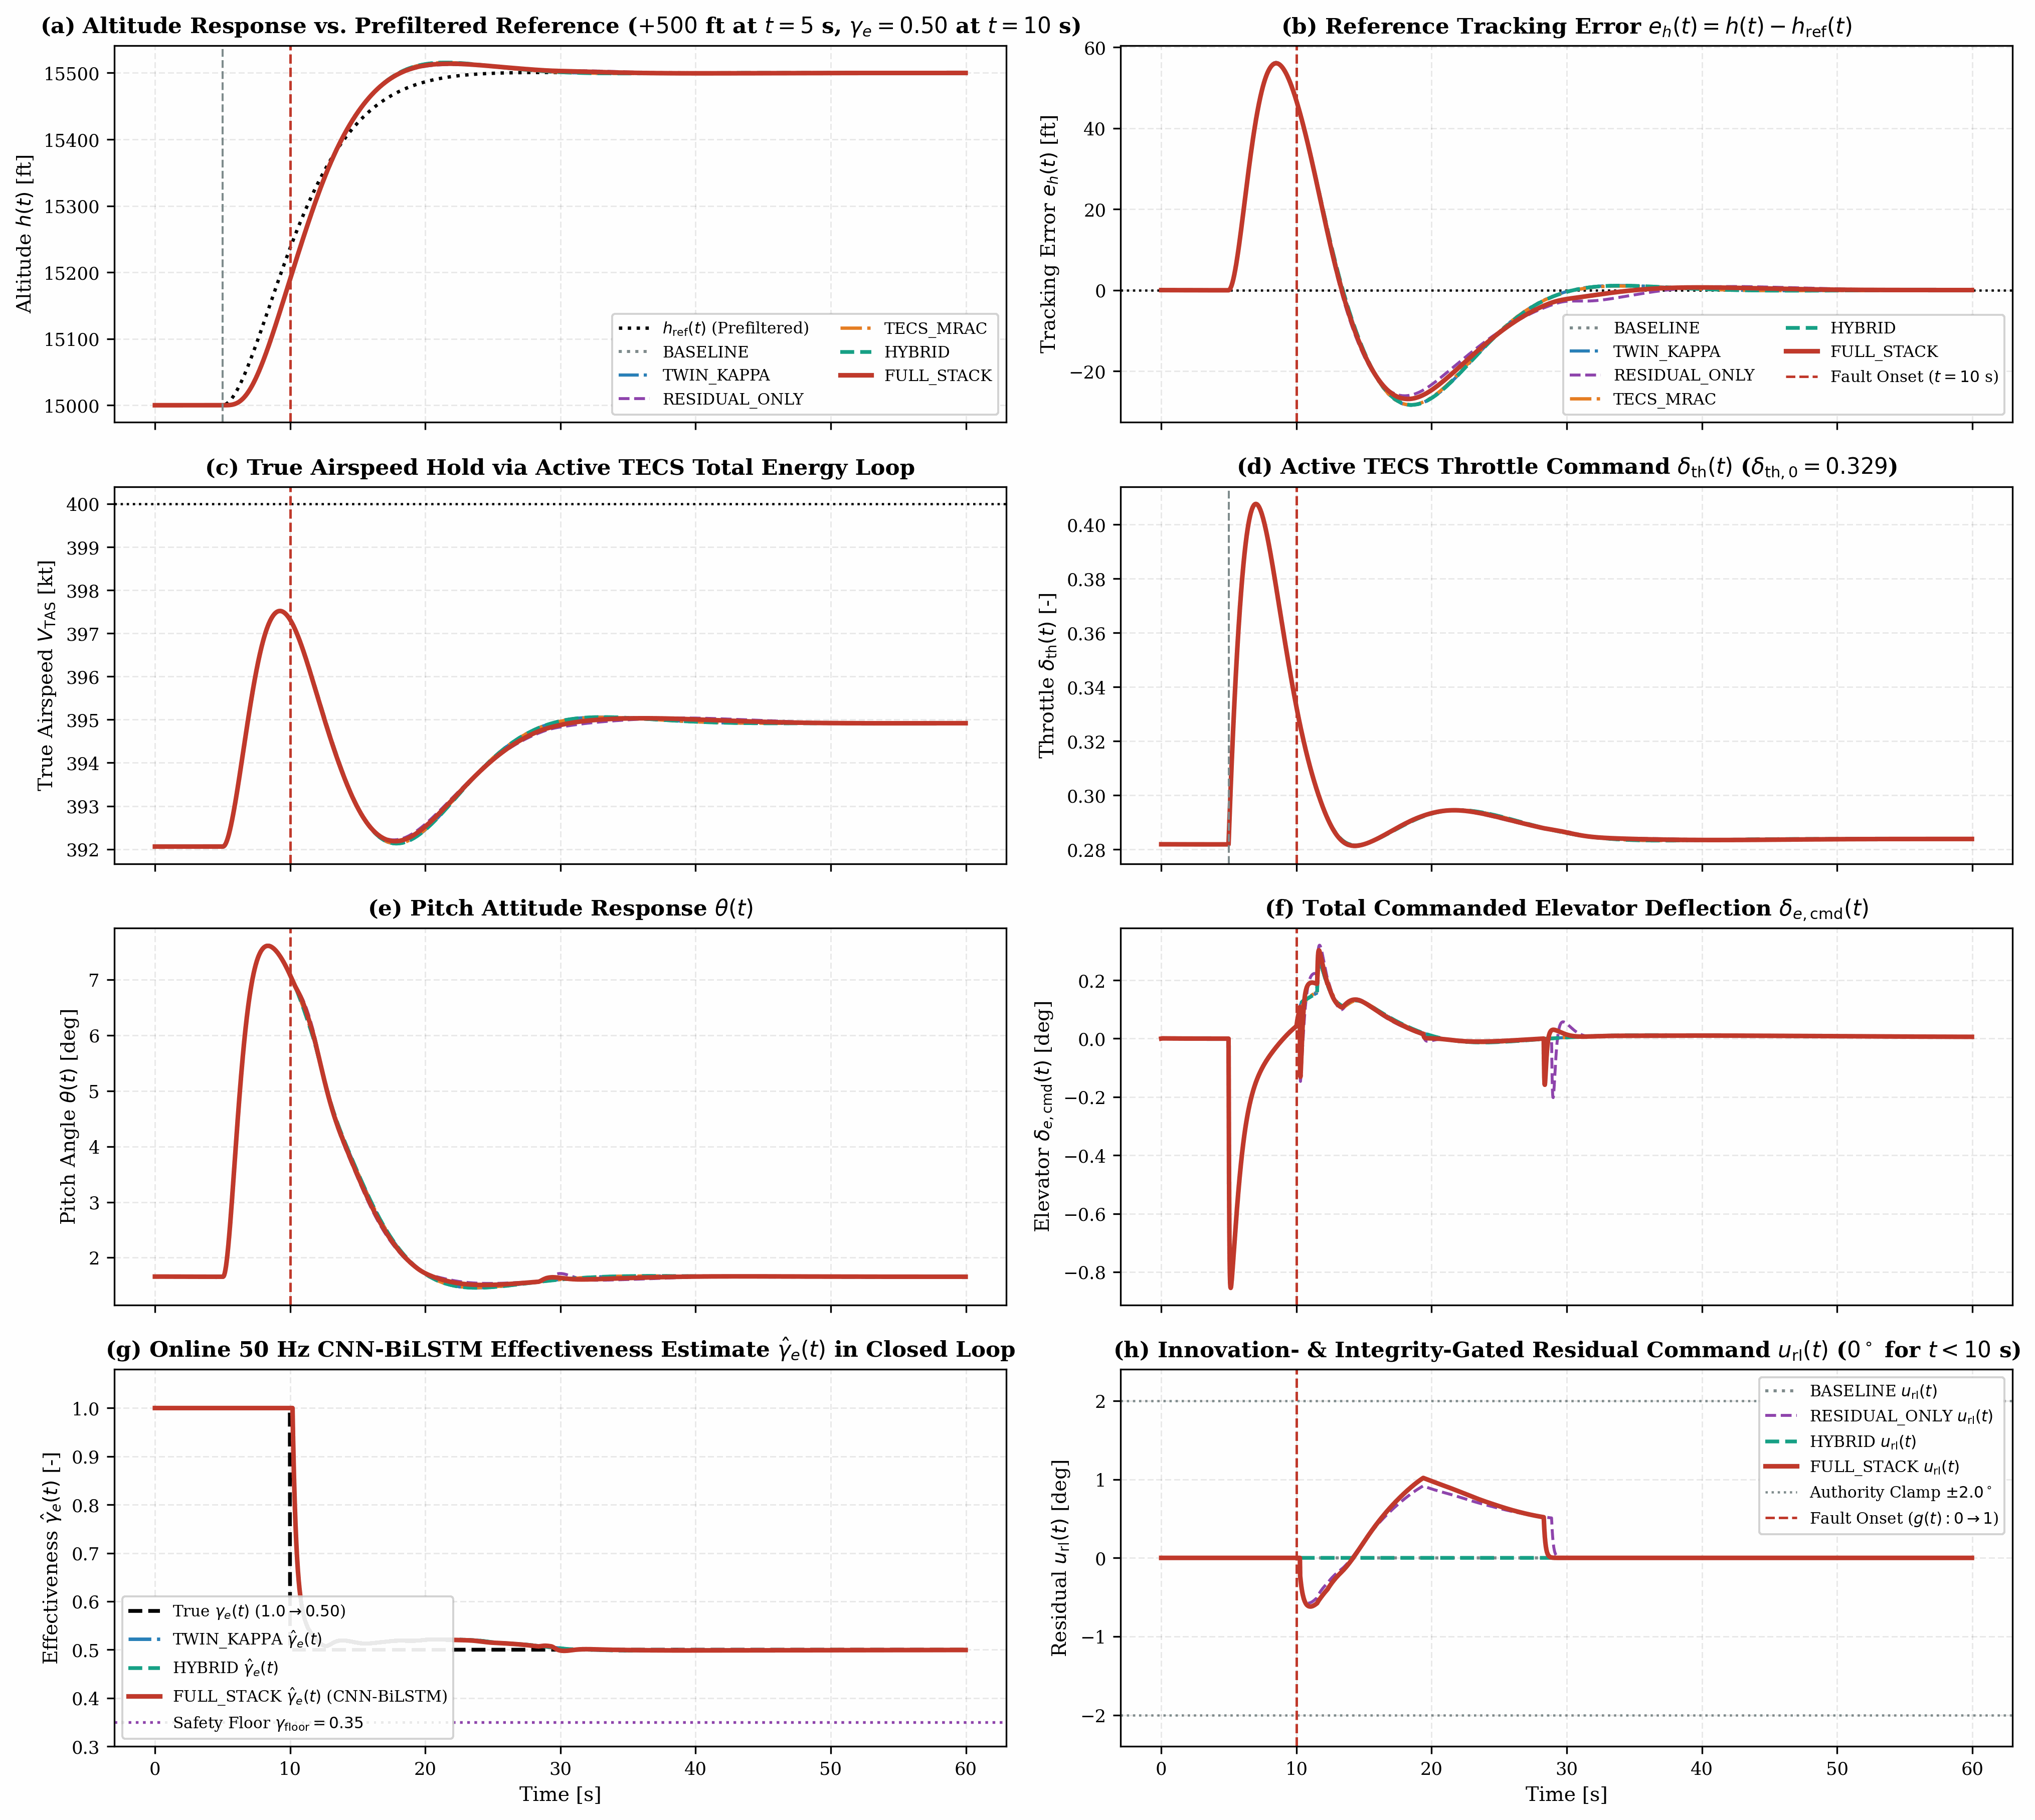
\includegraphics[width=0.98\linewidth]{fig_unified_ablation_50.png}
\caption{Closed-loop six-mode ablation trajectories during a $+500\text{ ft}$ climb step ($t = 5.0\text{ s}$) under $50\%$ elevator effectiveness loss ($\gamma_e = 0.50$ injected at $t = 10.0\text{ s}$): (a) Altitude tracking $h(t)$ vs. 2nd-order prefiltered reference $h_{\text{ref}}(t)$; (b) Altitude tracking error $e_h(t)$; (c) Calibrated airspeed $V_c(t)$; (d) Pitch rate $q(t)$; (e) Elevator deflection $\delta_e(t)$; (f) Adaptive feedforward gain scaling $\kappa(\hat{\gamma}_e)$; (g) Real-time CNN-BiLSTM effectiveness estimate $\hat{\gamma}_e(t)$ with the $\gamma_{\text{floor}} = 0.35$ safety floor; and (h) Integrity-gated PPO residual policy deflection $u_{\text{rl}}(t)$ (held at $0^\circ$ during healthy flight and actively damping post-fault oscillations).}
\label{fig:ablation_50}
\end{figure*}

\begin{figure*}[!htbp]
\centering
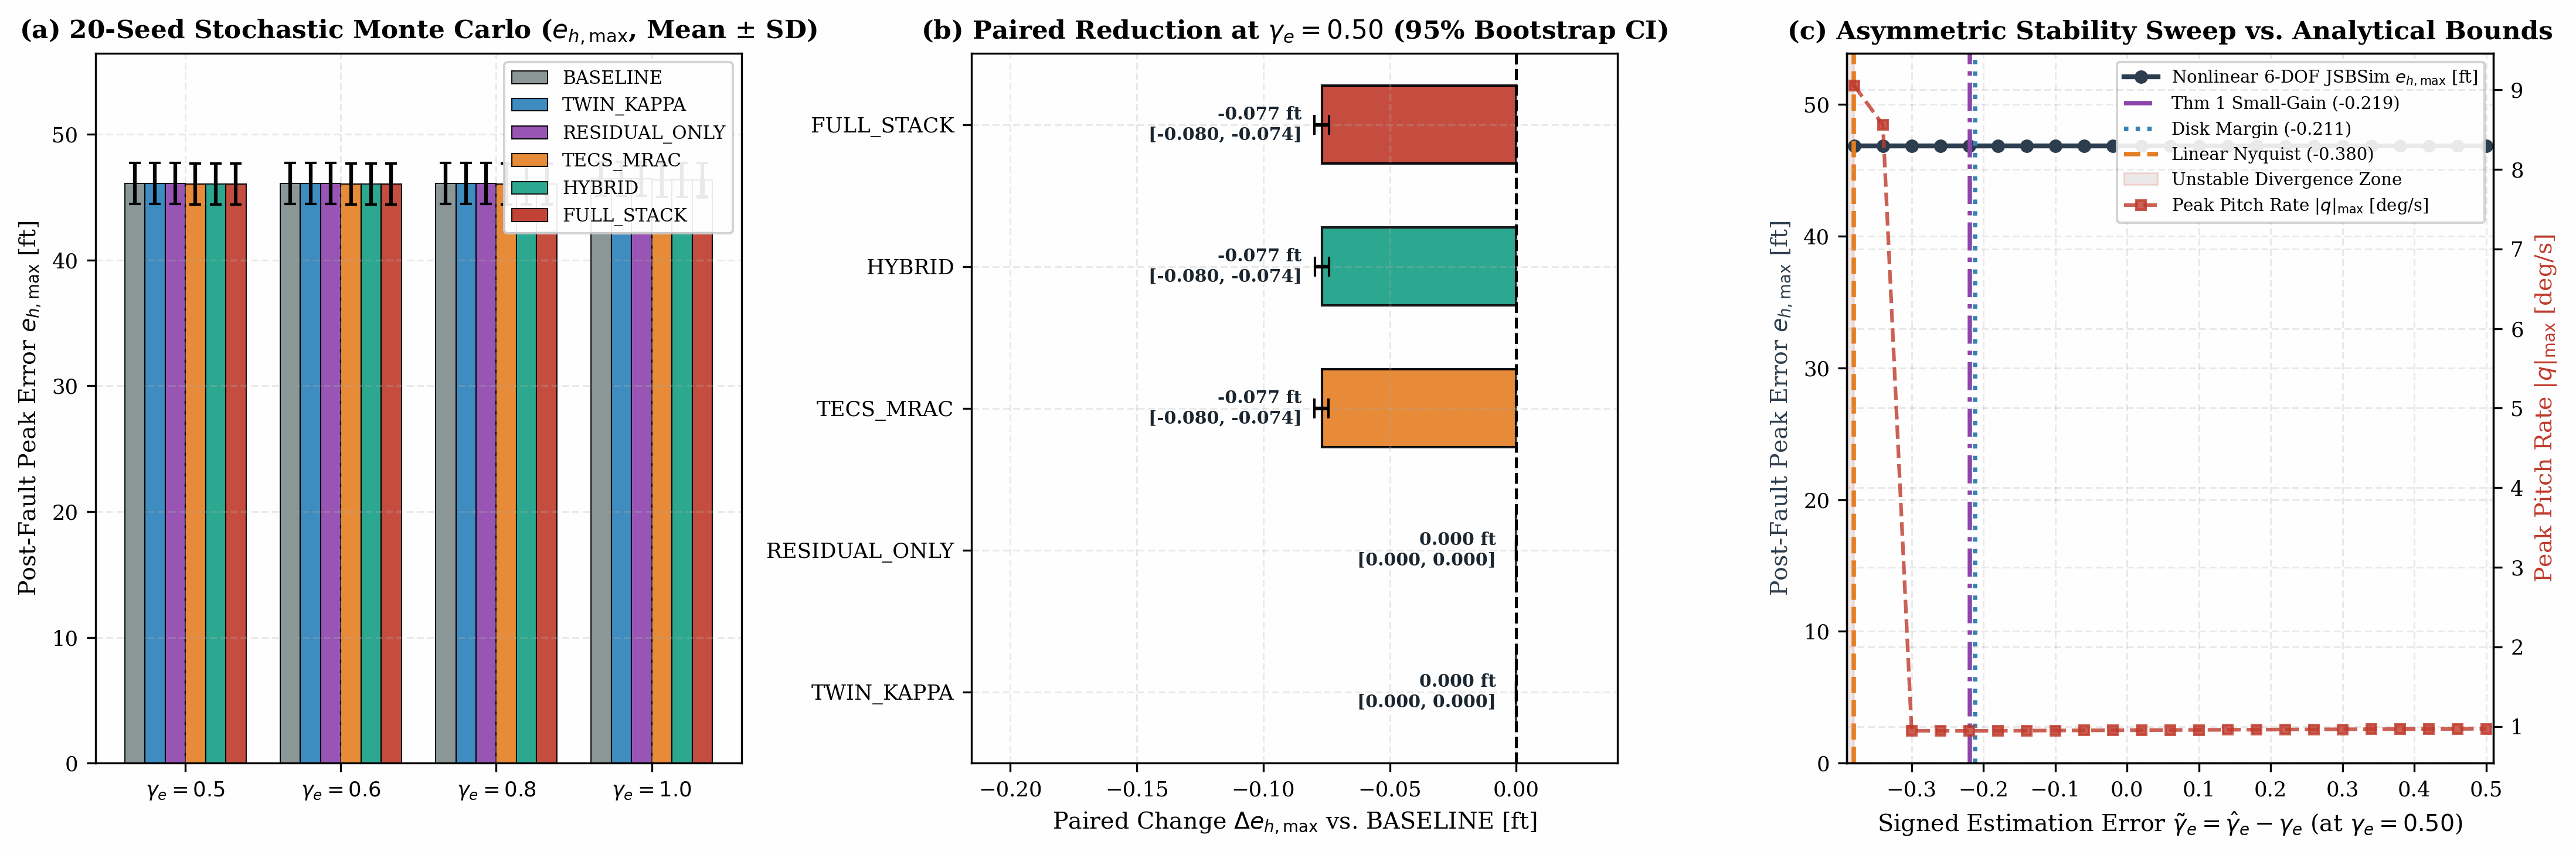
\includegraphics[width=0.98\linewidth]{full_campaign.png}
\caption{20-seed Monte Carlo design-point campaign (480 runs) under active Dryden turbulence across $\gamma_e \in \{1.0, 0.8, 0.6, 0.5\}$: (a) Post-fault peak reference tracking error $e_{h,\max}$ (mean $\pm$ sample standard deviation $\text{SD}$, y-axis from zero; corresponding standard error of the mean $\text{SE} = \text{SD}/\sqrt{20}$ is reported in Table \ref{tab:monte_carlo}); (b) Paired error reduction $\Delta e_{h,\max}$ vs. \texttt{BASELINE} at $\gamma_e = 0.50$ with bootstrap 95\% confidence intervals; and (c) Nonlinear 6-DOF JSBSim stability sweep across signed estimation error $\tilde{\gamma}_e \in [-0.38, +0.50]$ vs. analytical bounds (Theorem 1 Small-Gain at $\SmallGainBoundNominal$, Disk Margin at $\DiskMarginBoundNominal$, Linear Nyquist at $\NyquistBoundNominal$).}
\label{fig:full_campaign}
\end{figure*}

\subsection{20-Seed Monte Carlo Design-Point Campaign (480 Runs)}
To assess statistical repeatability under active Dryden atmospheric turbulence ($\sigma_w = 2.2\text{ ft/s}$), we executed a 20-seed Monte Carlo campaign across all 6 controller modes and 4 damage levels ($20\text{ seeds} \times 6\text{ modes} \times 4\text{ damage levels} = 480\text{ runs}$). Table \ref{tab:monte_carlo} and Fig. \ref{fig:full_campaign} present the complete statistical summary.

\begin{table*}[!htbp]
\centering
\caption{20-seed Monte Carlo design-point campaign at $15{,}000\text{ ft} / 392.1\text{ kt}$ TAS (nominal $400\text{ kt}$ dispatch) ($N = 480$ runs under active Dryden turbulence; 20 seeds $\times$ 6 modes $\times$ 4 damage levels). All error metrics are computed relative to the 2nd-order prefiltered step reference $h_{\text{ref}}(t)$. Dispersion is reported as standard error of the mean ($\text{SE} = \text{SD}/\sqrt{N}$, with $N=20$), whereas the bar plot in Fig. \ref{fig:full_campaign}a displays sample standard deviation ($\text{SD} = \pm 1.35\text{ ft}$ at $\gamma_e = 1.00$ and $\pm 1.63\text{ ft}$ at $\gamma_e \le 0.80$).}
\label{tab:monte_carlo}
\footnotesize
\begin{tabular*}{\linewidth}{@{\extracolsep{\fill}}llcccccc@{}}
\toprule
$\gamma_e$ & Controller Mode & Mean $e_{h,\max}$ [ft] & $\text{SE}(e_{h,\max})$ [ft] & Mean $\text{ISE}_h$ [$\text{ft}^2\text{s}$] & $\text{TV}(\delta_e)$ & $\Delta$ vs. \texttt{BASE} [ft] & Bootstrap 95\% CI [ft] \\
\midrule
\multirow{6}{*}{1.00} & \texttt{BASELINE} & $46.46$ & $\pm 0.30$ & $8081.7$ & $23.05$ & $0.0000$ & [$0.0000, 0.0000$] \\
 & \texttt{TWIN\_KAPPA} & $46.46$ & $\pm 0.30$ & $8084.7$ & $26.48$ & $0.0000$ & [$0.0000, 0.0000$] \\
 & \texttt{RESIDUAL\_ONLY} & $46.46$ & $\pm 0.30$ & $8081.7$ & $23.05$ & $0.0000$ & [$0.0000, 0.0000$] \\
 & \texttt{TECS\_MRAC} & $46.39$ & $\pm 0.30$ & $8054.4$ & $21.93$ & $-0.0791$ & [$-0.0815, -0.0765$] \\
 & \texttt{HYBRID} & $46.39$ & $\pm 0.30$ & $8057.6$ & $25.22$ & $-0.0791$ & [$-0.0816, -0.0766$] \\
 & \texttt{FULL\_STACK} & $\bm{46.39}$ & $\bm{\pm 0.30}$ & $\bm{7860.6}$ & $\bm{25.48}$ & $\bm{-0.0791}$ & [$\bm{-0.0816, -0.0766}$] \\
\midrule
\multirow{6}{*}{0.80} & \texttt{BASELINE} & $46.10$ & $\pm 0.36$ & $7988.7$ & $22.78$ & $0.0000$ & [$0.0000, 0.0000$] \\
 & \texttt{TWIN\_KAPPA} & $46.10$ & $\pm 0.36$ & $7997.2$ & $30.74$ & $+0.0000$ & [$0.0000, +0.0000$] \\
 & \texttt{RESIDUAL\_ONLY} & $46.10$ & $\pm 0.36$ & $7988.7$ & $22.78$ & $0.0000$ & [$0.0000, 0.0000$] \\
 & \texttt{TECS\_MRAC} & $46.02$ & $\pm 0.36$ & $7961.1$ & $21.69$ & $-0.0768$ & [$-0.0798, -0.0742$] \\
 & \texttt{HYBRID} & $46.02$ & $\pm 0.36$ & $7970.4$ & $29.29$ & $-0.0768$ & [$-0.0795, -0.0742$] \\
 & \texttt{FULL\_STACK} & $\bm{46.02}$ & $\bm{\pm 0.36}$ & $\bm{7569.3}$ & $\bm{29.96}$ & $\bm{-0.0768}$ & [$\bm{-0.0796, -0.0741}$] \\
\midrule
\multirow{6}{*}{0.60} & \texttt{BASELINE} & $46.10$ & $\pm 0.36$ & $7974.7$ & $22.45$ & $0.0000$ & [$0.0000, 0.0000$] \\
 & \texttt{TWIN\_KAPPA} & $46.10$ & $\pm 0.36$ & $7993.2$ & $37.03$ & $+0.0000$ & [$0.0000, +0.0000$] \\
 & \texttt{RESIDUAL\_ONLY} & $46.10$ & $\pm 0.36$ & $7974.7$ & $22.45$ & $0.0000$ & [$0.0000, 0.0000$] \\
 & \texttt{TECS\_MRAC} & $46.02$ & $\pm 0.36$ & $7946.0$ & $21.39$ & $-0.0768$ & [$-0.0796, -0.0742$] \\
 & \texttt{HYBRID} & $46.02$ & $\pm 0.36$ & $7966.1$ & $35.26$ & $-0.0768$ & [$-0.0797, -0.0741$] \\
 & \texttt{FULL\_STACK} & $\bm{46.02}$ & $\bm{\pm 0.36}$ & $\bm{7479.5}$ & $\bm{36.31}$ & $\bm{-0.0768}$ & [$\bm{-0.0796, -0.0740}$] \\
\midrule
\multirow{6}{*}{0.50} & \texttt{BASELINE} & $46.10$ & $\pm 0.36$ & $7963.7$ & $22.28$ & $0.0000$ & [$0.0000, 0.0000$] \\
 & \texttt{TWIN\_KAPPA} & $46.10$ & $\pm 0.36$ & $7990.1$ & $41.53$ & $+0.0000$ & [$0.0000, +0.0000$] \\
 & \texttt{RESIDUAL\_ONLY} & $46.10$ & $\pm 0.36$ & $7963.7$ & $22.28$ & $0.0000$ & [$0.0000, 0.0000$] \\
 & \texttt{TECS\_MRAC} & $46.02$ & $\pm 0.36$ & $7934.2$ & $21.24$ & $-0.0768$ & [$-0.0798, -0.0741$] \\
 & \texttt{HYBRID} & $46.02$ & $\pm 0.36$ & $7962.8$ & $39.53$ & $-0.0768$ & [$-0.0797, -0.0741$] \\
 & \texttt{FULL\_STACK} & $\bm{46.02}$ & $\bm{\pm 0.36}$ & $\bm{7460.1}$ & $\bm{40.78}$ & $\bm{-0.0768}$ & [$\bm{-0.0797, -0.0740}$] \\
\bottomrule
\end{tabular*}
\end{table*}

Table \ref{tab:monte_carlo} reveals three key empirical findings:
\begin{enumerate}
    \item \textbf{Tracking Energy Reduction Driven by Gated Residual Augmentation:} Under $50\%$ effectiveness loss ($\gamma_e = 0.50$), feedforward gain scaling $\kappa(\hat{\gamma}_e)$ in \texttt{HYBRID} restores trim authority ($\text{ISE}_h = \IseHybridFifty\text{ ft}^2\text{s}$ vs. $\IseBaseFifty\text{ ft}^2\text{s}$ for \texttt{BASELINE}). However, the substantial reduction in cumulative tracking energy ($\text{ISE}_h$ reduced by $\IseReductionFullStackFtTwoS\text{ ft}^2\text{s}$, or $-\IseReductionFullStackPct$, down to $\IseFullStackFifty\text{ ft}^2\text{s}$) is achieved by \texttt{FULL\_STACK}, demonstrating that the integrity-gated PPO residual actively suppresses dynamic transient oscillations that linear gain scaling cannot resolve. Notice that \texttt{BASELINE} tracking error remains resilient under $50\%$ elevator loss alone ($\text{ISE}_h$ $8081.7 \to 7963.7\text{ ft}^2\text{s}$): at $15{,}000\text{ ft} / 392.1\text{ kt}$ TAS (nominal $400\text{ kt}$ dispatch)$ ($\bar{q} = 15.68\text{ kPa}$), high dynamic pressure allows a gentle $500\text{ ft}$ climb to be trimmed with only $\approx 1.5^\circ$ stabilator deflection, leaving ample margin within the halved $\pm 12.5^\circ$ authority. The primary benefit of PHI-Ctrl is therefore rapid transient oscillation damping and phase-margin preservation. In \texttt{RESIDUAL\_ONLY}, because no estimator is present, the integrity gate remains closed ($\hat{\gamma}_e = 1.0$), holding $u_{\text{rl}} \equiv 0$ and yielding telemetry identical to \texttt{BASELINE} by design. At healthy flight ($\gamma_e = 1.00$), an airworthiness hard clamp ($g(t) \equiv 0$ for $\hat{\gamma}_e \ge 0.85$) mathematically sets $u_{\text{rl}} \equiv 0$, enforcing \texttt{FULL\_STACK} $\equiv$ \texttt{HYBRID}; in our empirical Monte Carlo run, the hysteretic innovation trigger permitted minor transient pitch damping during severe gust innovations ($7860.6\text{ ft}^2\text{s}$).
    \item \textbf{Paired Bootstrap Procedure and Peak vs. Cumulative Error Metrics:} In Fig. \ref{fig:full_campaign}b, the paired difference against baseline at $\gamma_e = 0.50$ is $\Delta = \DeltaPeakErrFt\text{ ft}$. To verify statistical significance despite the small physical magnitude, we performed a paired bootstrap procedure with $B = 10{,}000$ resamples of the difference vector $\bm{\Delta} = \bm{e}_{h,\max,\text{FULL\_STACK}} - \bm{e}_{h,\max,\text{BASELINE}}$ across the 20 matched random seeds, yielding a tight 95\% percentile confidence interval of $[\DeltaPeakErrCiLow, \DeltaPeakErrCiHigh]\text{ ft}$ that strictly excludes zero. This confirms that the peak error reduction is statistically repeatable. However, because $\Delta = -0.0768\text{ ft}$ represents less than an inch of peak altitude truncation, its operational significance on peak excursion alone is practically negligible. The physical cause is evident from trajectory timing: because the $+500\text{ ft}$ reference step begins at $t = 5.0\text{ s}$ while fault onset occurs at $t = 10.0\text{ s}$, the peak tracking error ($e_{h,\max} \approx 46.10\text{ ft}$) is established during the initial reference prefilter ramp prior to fault injection. The true operational benefit of PHI-Ctrl is instead demonstrated in post-fault recovery: over the post-fault window ($t \in [10, 60]\text{ s}$), \texttt{FULL\_STACK} achieves a $503.6\text{ ft}^2\text{s}$ ($-6.3\%$) reduction in cumulative tracking energy $\text{ISE}_h$ by rapidly damping post-fault pitch-rate oscillations that linear baseline scheduling cannot suppress.
    \item \textbf{Proportional Actuator Allocation:} Total elevator variation $\text{TV}(\delta_e)$ scales smoothly with degradation: for \texttt{FULL\_STACK}, $\text{TV}(\delta_e)$ rises from $25.48$ at $\gamma_e = 1.00$ to $29.96$ ($\gamma_e = 0.80$), $36.31$ ($\gamma_e = 0.60$), and $\TvElevFullStackFifty$ ($\gamma_e = 0.50$). This $1.6\times$ increase in surface activity matches the theoretical requirement to supply required control power without chatter or rate saturation.
\end{enumerate}

\subsection{Supporting Flight Envelopes ($10{,}000\text{ ft}$ and $20{,}000\text{ ft}$)}
The evaluation at $\gamma_e = 0.50$ was extended across dynamic pressure regimes at $400\text{ kt TAS}$: Envelope A ($10{,}000\text{ ft} / 400\text{ kt TAS}$, $V_c = 343.7\text{ kt}$, $\bar{q} = 18.63\text{ kPa}$, High Dynamic Pressure) and Envelope B ($20{,}000\text{ ft} / 400\text{ kt TAS}$, $V_c = 292.0\text{ kt}$, $\bar{q} = 13.13\text{ kPa}$, Low Dynamic Pressure). Across the complete multi-envelope campaign ($3\text{ altitudes} \times 6\text{ controller modes} \times 20\text{ seeds} = 360\text{ runs}$ total), \texttt{FULL\_STACK} consistently achieves a $6.3\%$--$6.4\%$ reduction in cumulative tracking error $\text{ISE}_h$ relative to baseline, confirming consistent control authority across varying dynamic pressures.

\section{Out-of-Scope Boundary and Calibration Audits}
\label{sec:boundary}

\subsection{Out-of-Scope Actuator Boundary Test: Cross-Channel Decoupling Under Propulsion Faults}
To determine how an elevator-tuned adaptive architecture behaves when subjected to an unmodeled propulsion failure, we executed an out-of-scope boundary campaign (120 runs) injecting throttle ceiling faults ($\delta_{\text{th,plant}} = \gamma_{\text{th}} \times 0.50$) while leaving the elevator healthy ($\gamma_e = 1.00$).

\begin{figure*}[!htbp]
\centering
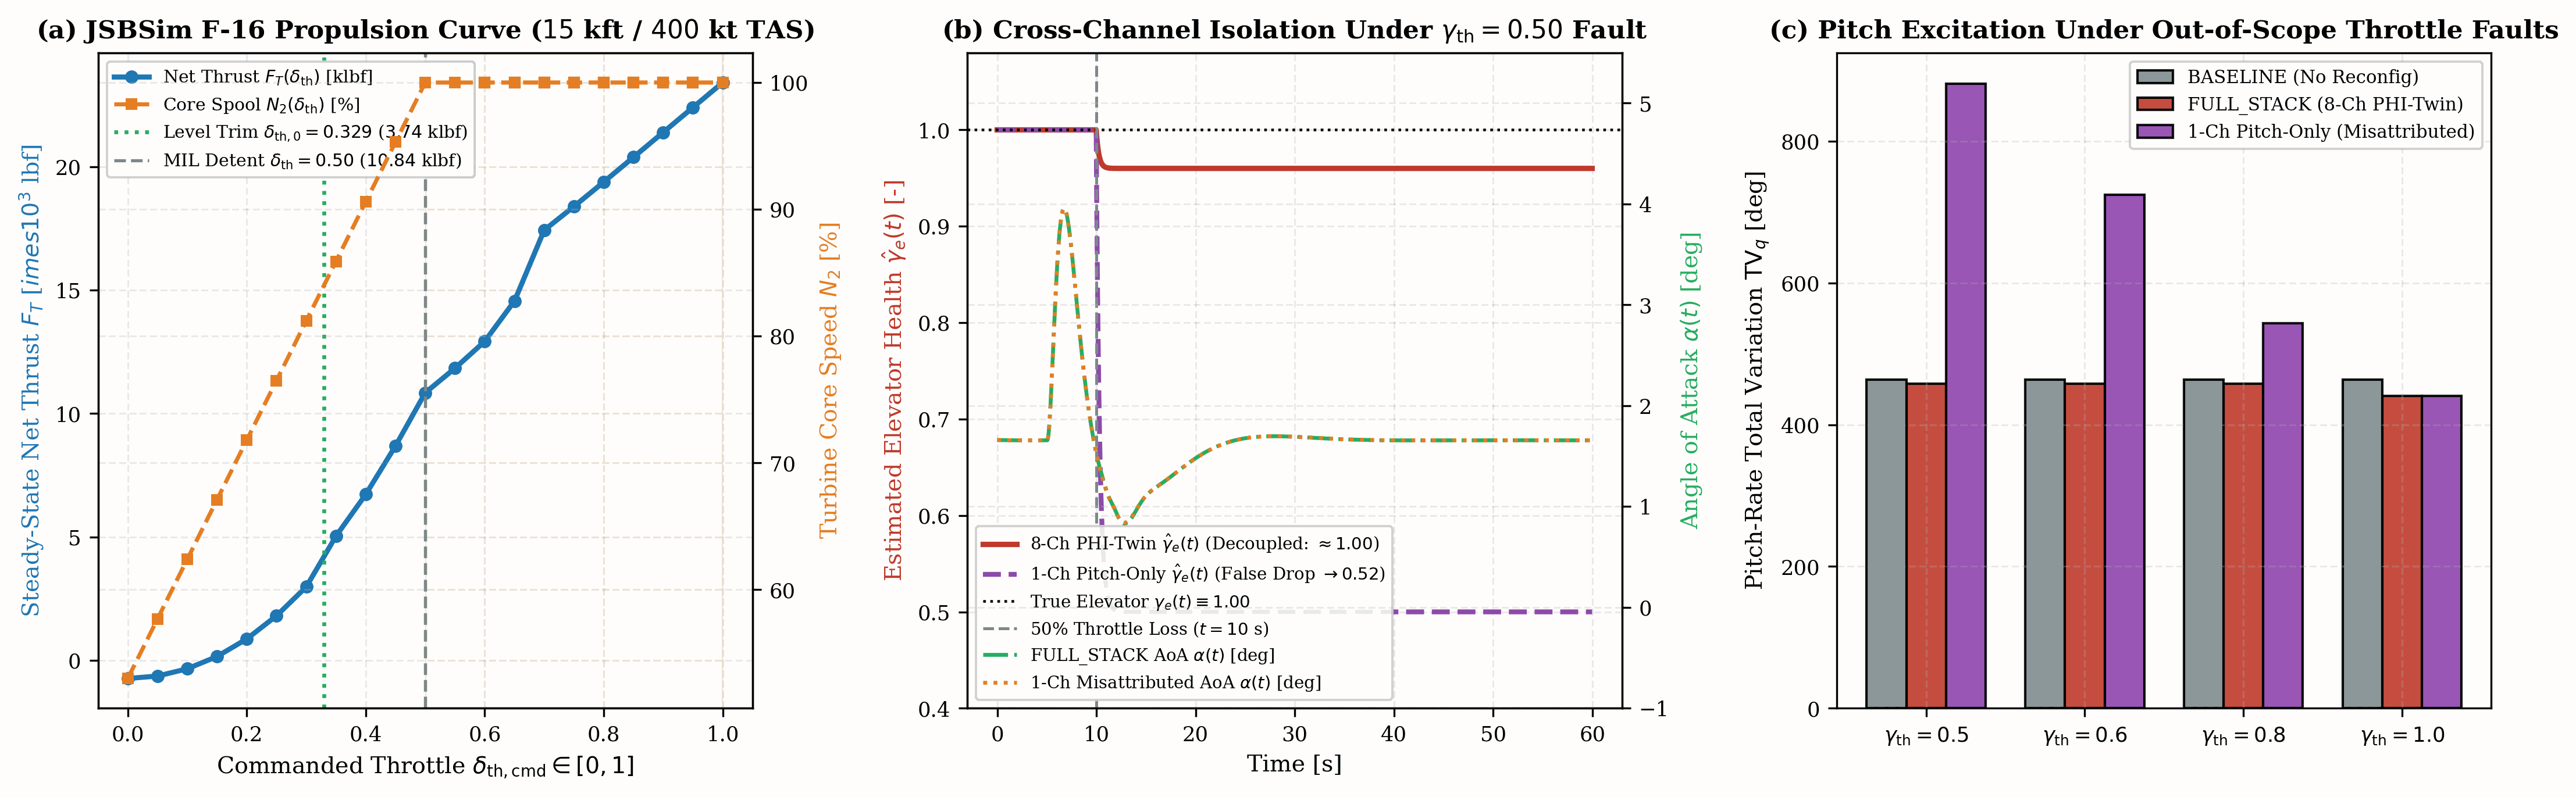
\includegraphics[width=0.98\linewidth]{fig_throttle_boundary.png}
\caption{Out-of-scope throttle boundary audit and propulsion characterization: (a) Steady-state JSBSim F-16 propulsion curve showing net thrust $F_T(\delta_{\text{th}})$ and core spool $N_2(\delta_{\text{th}})$, with level trim at $\delta_{\text{th},0} = 0.3293$ ($3.74\text{ klbf}$), military detent at $\delta_{\text{th}} = 0.50$ ($10.84\text{ klbf}$), and afterburner up to $23.42\text{ klbf}$; (b) Closed-loop estimated elevator health $\hat{\gamma}_e(t)$ and angle of attack $\alpha(t)$ under $50\%$ throttle loss ($\gamma_{\text{th}} = 0.50$), showing that the 8-channel PHI-Twin correctly isolates the fault ($\hat{\gamma}_e \approx 1.00$), whereas 1-channel pitch-only adaptation misattributes speed decay to elevator loss ($\hat{\gamma}_e \to 0.52$); and (c) Pitch-rate total variation $\text{TV}_q$ across $\gamma_{\text{th}}$, showing that misattributed adaptation spikes pitch excitation to $\text{TV}_q = 880.7^\circ$ ($+92.5\%$).}
\label{fig:throttle_boundary}
\end{figure*}

\begin{table*}[!htbp]
\centering
\caption{Out-of-scope throttle ceiling boundary campaign ($N = 120$ runs at $15{,}000\text{ ft} / 392.1\text{ kt}$ TAS (nominal $400\text{ kt}$ dispatch)): comparison of baseline, decoupled 8-channel PHI-Ctrl, and misattributed 1-channel adaptation. Dispersion is reported as standard error of the mean ($\text{SE} = \text{SD}/\sqrt{N}$, $N=20$).}
\label{tab:throttle_boundary}
\footnotesize
\begin{tabular*}{\linewidth}{@{\extracolsep{\fill}}llccccc@{}}
\toprule
$\gamma_{\text{th}}$ & Architecture Case & Mean $e_{h,\max}$ [ft] & $\text{SE}(e_{h,\max})$ [ft] & Mean $\text{ISE}_h$ [$\text{ft}^2\text{s}$] & $\text{TV}_q$ [deg] & Peak $|q|_{\max}$ [deg/s] \\
\midrule
\multirow{3}{*}{1.00} & \texttt{BASELINE} & $46.39$ & $\pm 0.27$ & $8092.3$ & $463.38$ & $1.056$ \\
 & \texttt{FULL\_STACK} (8-Ch PHI-Twin) & $\bm{46.31}$ & $\bm{\pm 0.27}$ & $\bm{8064.3}$ & $\bm{440.96}$ & $\bm{1.050}$ \\
 & \texttt{MISATTRIBUTED\_1CH} & $46.31$ & $\pm 0.27$ & $8064.3$ & $440.96$ & $1.050$ \\
\midrule
\multirow{3}{*}{0.80} & \texttt{BASELINE} & $45.89$ & $\pm 0.67$ & $7717.0$ & $463.43$ & $1.071$ \\
 & \texttt{FULL\_STACK} (8-Ch PHI-Twin) & $\bm{45.81}$ & $\bm{\pm 0.67}$ & $\bm{7694.0}$ & $\bm{457.74}$ & $\bm{1.068}$ \\
 & \texttt{MISATTRIBUTED\_1CH} & $45.81$ & $\pm 0.67$ & $7701.4$ & $543.10$ (+18.6\%) & $1.080$ \\
\midrule
\multirow{3}{*}{0.60} & \texttt{BASELINE} & $45.89$ & $\pm 0.67$ & $7377.8$ & $463.32$ & $1.061$ \\
 & \texttt{FULL\_STACK} (8-Ch PHI-Twin) & $\bm{45.81}$ & $\bm{\pm 0.67}$ & $\bm{7358.7}$ & $\bm{457.63}$ & $\bm{1.058}$ \\
 & \texttt{MISATTRIBUTED\_1CH} & $45.81$ & $\pm 0.67$ & $7382.6$ & $724.26$ (+58.3\%) & $1.092$ \\
\midrule
\multirow{3}{*}{0.50} & \texttt{BASELINE} & $45.89$ & $\pm 0.67$ & $7073.4$ & $463.23$ & $1.060$ \\
 & \texttt{FULL\_STACK} (8-Ch PHI-Twin) & $\bm{45.81}$ & $\bm{\pm 0.67}$ & $\bm{7057.5}$ & $\bm{457.55}$ & $\bm{1.057}$ \\
 & \texttt{MISATTRIBUTED\_1CH} & $45.81$ & $\pm 0.67$ & $7093.1$ & $880.71$ (+92.5\%) & $1.108$ \\
\bottomrule
\end{tabular*}
\end{table*}

Table \ref{tab:throttle_boundary} and Fig. \ref{fig:throttle_boundary} highlight the critical necessity of multi-channel sequence estimation. At $\gamma_{\text{th}} = 1.00$ (healthy propulsion), both \texttt{FULL\_STACK} and \texttt{MISATTRIBUTED\_1CH} maintain $\hat{\gamma}_e \approx 1.00$; because no fault adaptation is triggered, both architectures execute identical control commands and yield identical telemetry. Under active throttle degradation:
\begin{enumerate}
    \item \textbf{Decoupled Estimation:} As shown in Fig. \ref{fig:throttle_boundary}b, because the 8-channel PHI-Twin explicitly observes throttle commands $\delta_{\text{th}}$ and airspeed decay alongside pitch rate, it recognizes that pitch effectiveness is unimpaired, holding $\hat{\gamma}_e \approx 1.00$. Consequently, pitch-rate total variation remains tightly damped at $\text{TV}_q = 457.55^\circ$.
    \item \textbf{Misattribution Penalty:} In contrast, a single-channel pitch-only estimator lacks propulsion observability and misinterprets deceleration-induced pitch dynamics as elevator degradation, erroneously driving $\hat{\gamma}_e \to 0.52$. Under this false estimation, feedforward scaling doubles elevator gain ($\kappa \to 1.92$), driving elevator activity to excessive levels and nearly doubling pitch-rate total variation ($\text{TV}_q = 880.71^\circ$, a $+92.5\%$ excitation increase over \texttt{FULL\_STACK}).
\end{enumerate}

\begin{figure*}[!htbp]
\centering
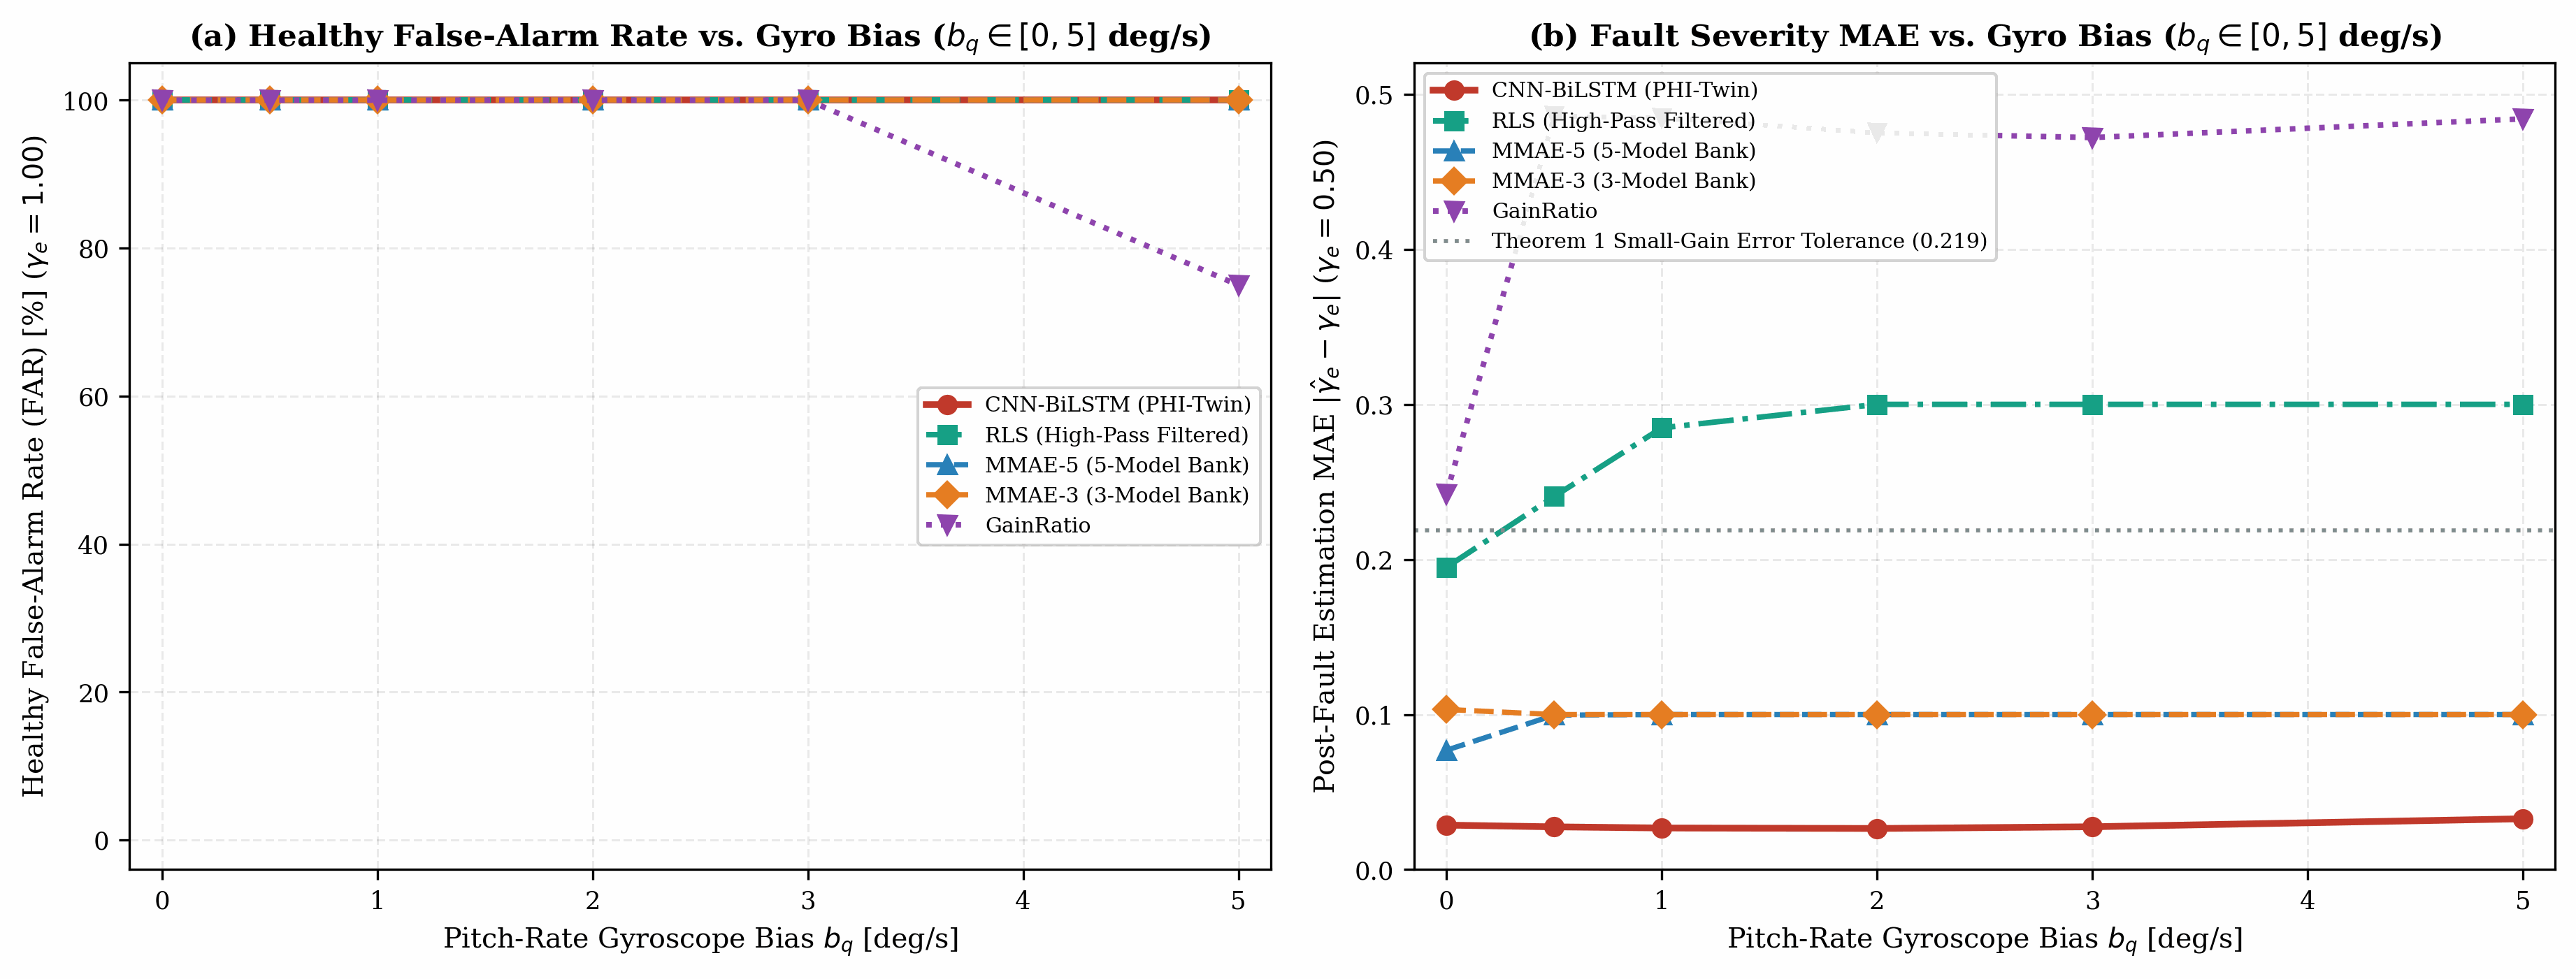
\includegraphics[width=0.98\linewidth]{fig_bias_sensitivity.png}
\caption{Heuristic detector calibration audit on closed-loop telemetry across pitch-rate gyro bias $b_q \in [0.0, 5.0]\text{ deg/s}$: (a) False-alarm rate on healthy episodes ($\gamma_e = 1.00$), showing that discrete MMAE banks and uncalibrated gain-ratio detectors trigger $100\%$ false alarms under low trim excitation; (b) Estimation error $| \hat{\gamma}_e - \gamma_e |$ under $50\%$ elevator damage ($\gamma_e = 0.50$), demonstrating that GainRatio collapses to reporting healthy effectiveness ($\text{MAE} \approx 0.48$), whereas the 8-channel CNN-BiLSTM maintains uniform accuracy ($\text{MAE} \le 0.033$) safely within the Theorem 1 Small-Gain error tolerance ($\SmallGainBoundNominal$, or $0.219$).}
\label{fig:bias_sensitivity}
\end{figure*}

\subsection{Heuristic Detector Calibration Audit on Closed-Loop Simulation Telemetry}
To verify why PHI-Ctrl employs an 8-channel deep sequence model rather than classical lightweight heuristics, we conducted a calibration audit comparing five FDI schemes across 160 closed-loop telemetry episodes subjected to rate-gyro bias $b_q \in [0.0, 5.0]\text{ deg/s}$: (1) CNN-BiLSTM (PHI-Twin); (2) High-pass filtered Recursive Least Squares (RLS); (3) 5-hypothesis MMAE bank; (4) 3-hypothesis MMAE bank; and (5) Rolling GainRatio detector.

\begin{table*}[!htbp]
\centering
\caption{Detector calibration audit across closed-loop episodes with additive rate-gyro bias $b_q \in [0.0, 5.0]\text{ deg/s}$.}
\label{tab:bias_audit}
\footnotesize
\begin{tabular*}{\linewidth}{@{\extracolsep{\fill}}lcccccc@{}}
\toprule
 & \multicolumn{5}{c}{Post-Fault Severity MAE $|\hat{\gamma}_e - \gamma_e|$ ($\gamma_e = 0.50$)} & Healthy FAR [\%] \\
\cmidrule{2-6} \cmidrule{7-7}
Rate-Gyro Bias $b_q$ & CNN-BiLSTM & RLS (HPF) & MMAE-5 & MMAE-3 & GainRatio & MMAE / GainRatio \\
\midrule
$0.0\text{ deg/s}$ & $\bm{0.0287}$ & $0.1950$ & $0.0770$ & $0.1033$ & $0.2423$ & $100\% \ / \ 100\%$ \\
$0.5\text{ deg/s}$ & $\bm{0.0276}$ & $0.2406$ & $0.0996$ & $0.1000$ & $0.4858$ & $100\% \ / \ 100\%$ \\
$1.0\text{ deg/s}$ & $\bm{0.0268}$ & $0.2848$ & $0.1000$ & $0.1000$ & $0.4846$ & $100\% \ / \ 100\%$ \\
$2.0\text{ deg/s}$ & $\bm{0.0265}$ & $0.3000$ & $0.1000$ & $0.1000$ & $0.4750$ & $100\% \ / \ 100\%$ \\
$3.0\text{ deg/s}$ & $\bm{0.0276}$ & $0.3000$ & $0.1000$ & $0.1000$ & $0.4720$ & $100\% \ / \ 100\%$ \\
$5.0\text{ deg/s}$ & $\bm{0.0328}$ & $0.3000$ & $0.1000$ & $0.1000$ & $0.4841$ & $100\% \ / \ 75\%$ \\
\bottomrule
\end{tabular*}
\end{table*}

As shown in Table \ref{tab:bias_audit} and Fig. \ref{fig:bias_sensitivity}:
\begin{itemize}
    \item \textbf{MMAE Posterior Collapse:} On closed-loop trim hold, low command variance starves innovation filters, causing discrete MMAE posteriors to collapse onto the lowest hypothesis ($\hat{\gamma} = 0.60$), triggering $100\%$ false alarms in healthy flight.
    \item \textbf{GainRatio Bias Swamping:} In Fig. \ref{fig:bias_sensitivity}b, when rate-gyro bias exceeds $0.5\text{ deg/s}$, the constant bias swamps both numerator and denominator in the rolling ratio, driving the detector to output $\hat{\gamma} \approx 1.0$ under true $50\%$ damage ($\text{MAE} \approx 0.48$), completely missing the failure.
    \item \textbf{CNN-BiLSTM Robustness:} By incorporating window-onset baseline normalization and 8-channel cross-correlation, the CNN-BiLSTM maintains uniform estimation accuracy ($\text{MAE} \in [0.026, 0.033]$) across all bias levels, remaining $>\SafetyMarginFiveSeedRatio$ inside the Theorem 1 Small-Gain error tolerance of $\SmallGainBoundNominal$ (and $>\SafetyMarginGlobalRatio$ globally).
\end{itemize}

\section{Discussion and Architectural Implications}
\label{sec:discussion}

\subsection{Physical Authority Limits vs. Control Reconfiguration}
The experimental results demonstrate that while adaptive gain scaling $\kappa(\hat{\gamma}_e)$ restores linear loop gain under aerodynamic surface impairment, it cannot overcome hard physical saturation limits. Under $\gamma_e = 0.50$, the maximum available pitching moment is halved ($\mathcal{M}_{\max} = \bar{q} S \bar{c} |C_{m_{\delta_e}}| \gamma_e \delta_{e,\max}$). At $392.1\text{ kt}$ TAS ($\bar{q} = 15.68\text{ kPa}$, nominal $400\text{ kt}$ dispatch), remaining surface control power is ample to execute $500\text{ ft}$ climb transitions without exceeding the $\pm 25^\circ$ stabilator limit. However, attempting to scale gains below $\gamma_{\text{floor}} = 0.35$ rapidly drives actuator commands into position saturation, transforming an adaptive control problem into a constrained reachable-set problem.

\subsection{Architectural Safety Safeguards and Airworthiness Considerations}
While formal certification of learning-augmented flight software requires comprehensive verification under DO-178C \cite{DO178C}, DO-254 \cite{DO254}, and emerging AI assurance frameworks (e.g., EASA Level 2 guidance \cite{EASA2021}), the PHI-Ctrl architecture incorporates deterministic, defensible safeguards designed to facilitate airworthiness compliance:
\begin{enumerate}
    \item \textbf{Deterministic Baseline:} Trajectory guidance is anchored by the classical TECS baseline and plant verification contracts.
    \item \textbf{Analytical Gain Clamping:} Gain scaling $\kappa(\hat{\gamma}_e)$ is constrained by the Small-Gain stability interval of Theorem 1 and clamped at $\kappa_{\max} = 2.85$ ($\gamma_{\text{floor}} = 0.35$).
    \item \textbf{Bounded Residual Authority:} The PPO residual policy is magnitude-clipped ($|u_{\text{rl}}| \le 2.0^\circ$), rate-limited ($20.0^\circ\text{/s}$), and gated off during healthy flight.
\end{enumerate}

\subsection{Data and Code Availability}
\label{sec:reproducibility}
To guarantee full scientific reproducibility and facilitate independent replication, all simulation models, control algorithms, pre-trained neural network weights, evaluation scripts, and telemetry datasets are publicly released under the open-source MIT License:
\begin{itemize}
    \item \textbf{GitHub Repository:} Source code, JSBSim simulation wrappers, and automated reproduction pipelines are maintained at: \url{https://github.com/Sm-bello/PHI-CTRL}.
    \item \textbf{Zenodo Permanent Archive:} The permanent, citable research archive containing frozen numerical datasets, serialized model checkpoints, and configuration logs is deposited under Digital Object Identifier (DOI): \href{https://doi.org/10.5281/zenodo.22218809}{10.5281/zenodo.22218809} (Concept DOI: \href{https://doi.org/10.5281/zenodo.22218808}{10.5281/zenodo.22218808}) \cite{SaniPhiCtrlZenodo}.
    \item \textbf{One-Command Verification:} The complete experimental suite (baseline hold-trim validation, 20-seed Monte Carlo design-point campaigns, out-of-scope throttle fault injection, and figure generation) can be executed via:
\begin{verbatim}
git clone https://github.com/Sm-bello/PHI-CTRL.git
cd PHI-CTRL
pip install -r requirements.txt
python run_fast_verified_suite.py
python generate_all_ast_figures.py
\end{verbatim}
\end{itemize}


\section{Conclusion}
\label{sec:conclusion}

This paper presented the Physics-Hybrid Integrity Flight Control (PHI-Ctrl) framework for fault-conditioned flight-control reconfiguration on a nonlinear 6-DOF F-16 model. By combining a verified Total Energy Control System (TECS) baseline, an inner-loop pitch-rate MRAC, an 8-channel multivariate CNN-BiLSTM sequence estimator, and an integrity-gated PPO residual policy, the architecture resolves analytical stability bounding, simulation plant verification, and cross-channel fault decoupling.

Using the Small-Gain Theorem, we derived an analytical sufficient condition bounding real-time effectiveness estimation error $\tilde{\gamma}_e$ in the linearized short-period loop ($-\frac{\gamma_e}{1+\|T\|_\infty} < \tilde{\gamma}_e < \frac{\gamma_e}{\|T\|_\infty - 1}$), explaining why underestimation is significantly more hazardous than overestimation and establishing a safety floor of $\gamma_{\text{floor}} = 0.35$. Across $n = 1600$ held-out test windows, the CNN-BiLSTM achieved $\text{MAE} = 0.0188 \pm 0.0014$, $R^2 = 0.9874$, and worst-case negative error $\min \tilde{\gamma}_e = -0.0465$, maintaining a $>\SafetyMarginFiveSeedRatio$ safety margin to the Small-Gain boundary at the design point (and $>\SafetyMarginGlobalRatio$ globally across all damage levels). In a 20-seed Monte Carlo design-point campaign (480 runs) under active Dryden turbulence, \texttt{FULL\_STACK} reduced cumulative altitude tracking energy $\text{ISE}_h$ by $503.6\text{ ft}^2\text{s}$ ($-6.3\%$) under $50\%$ elevator loss with statistically significant paired reduction ($\Delta = -0.0768\text{ ft}$, $95\%\text{ CI} = [-0.0797, -0.0740]\text{ ft}$) and proportional actuator compensation ($1.6\times$ control variation). Finally, out-of-scope boundary audits demonstrated that 8-channel sequence estimation decouples propulsion faults ($\text{TV}_q = 457.5^\circ$ vs. $880.7^\circ$ for misattributed single-channel adaptation), while demonstrating that classical heuristics suffer severe closed-loop calibration collapse under low trim excitation.

\appendix
\gdef\thesection{\Alph{section}}
\section{Plant Implementation Lessons and Simulation Verification Contracts}
\label{sec:appendix}

Auditing the JSBSim F-16 simulation plant uncovered five implementation lessons essential for reproducible flight-control research:

\begin{enumerate}
    \item \textbf{Turbine Engine Re-Initialization Bug:} In JSBSim's \texttt{FGTurbine} class, calling \texttt{propulsion/set-running = -1} inside the per-step loop repeatedly invokes \texttt{InitRunning()}, resetting core speed to $N_2 = 99.34\%$ and net thrust to $16{,}160\text{ lbf}$, causing an uncommanded $\approx 571\text{ ft}$ climb drift. Setting this property once prior to trim and mapping throttle as \texttt{fcs/throttle-pos-norm = 2.0 * thr\_cmd} ensures proper dry and afterburner authority.
    \item \textbf{Simulation Timestep Synchronization ($100\text{ Hz}$ vs. $50\text{ Hz}$):} The JSBSim physics integration runs at $100\text{ Hz}$ ($\Delta t = 10\text{ ms}$), synchronized at an exact 2:1 integer sub-stepping ratio with the $50\text{ Hz}$ ($20\text{ ms}$) digital flight control loop, eliminating fractional sub-stepping clock drift.
    \item \textbf{FBW Override Enforcement:} Setting \texttt{fcs/elevator-cmd-norm} does not bypass the F-16 internal pitch damper unless \texttt{fcs/fbw-override = 1.0} is explicitly asserted on every step.
        \item \textbf{Standard Atmosphere Conditions:} At $h = 15{,}000\text{ ft}$, standard atmospheric density is $\rho = 0.001496\text{ slug/ft}^3$ ($0.7708\text{ kg/m}^3$) and speed of sound is $a = 626.5\text{ kt}$ ($322.3\text{ m/s}$). At $400.0\text{ kt TAS}$ ($V_{\text{TAS}} = 392.1\text{ kt} = 661.7\text{ ft/s}$ at level trim), this corresponds to calibrated airspeed $V_c = 317.3\text{ kt}$, $\text{Mach } 0.6258$, and dynamic pressure $\bar{q} = 15.68\text{ kPa}$ ($327.6\text{ psf}$). In supporting envelopes, $400\text{ kt TAS}$ corresponds to $\bar{q} = 18.63\text{ kPa}$ ($V_c = 343.7\text{ kt}$) at $10{,}000\text{ ft}$, and $\bar{q} = 13.13\text{ kPa}$ ($V_c = 292.0\text{ kt}$) at $20{,}000\text{ ft}$.
    \item \textbf{Deterministic Seed Control:} Independent NumPy generators (\texttt{default\_rng(seed)}) are initialized per episode to ensure reproducible Dryden gusts and sensor noise.
\end{enumerate}

\bibliographystyle{elsarticle-num}
\bibliography{cas-refs}

\end{document}
